% ============================================================
% Compiler Design Lab Project Report — Review 3 (final)
% VIT Template | A4 | Times New Roman | 1.5 spacing
% Figures are in report_figures/ (upload that folder with this file).
% ============================================================
\documentclass[12pt,a4paper]{report}

% ---------- geometry (1.5" left for binding, 1" others) ----------
\usepackage[left=1.5in, right=1in, top=1in, bottom=1in]{geometry}

% ---------- font: Times New Roman equivalent ----------
\usepackage{mathptmx}
\usepackage[T1]{fontenc}

% ---------- spacing ----------
\usepackage{setspace}
\onehalfspacing

% ---------- graphics, tables, code ----------
\usepackage{graphicx}
\usepackage{booktabs}
\usepackage{tabularx}
\usepackage{float}
\usepackage{caption}
\captionsetup{font=footnotesize}

% ---------- listings for source code ----------
\usepackage{listings}
\usepackage{xcolor}
\lstset{
  basicstyle=\ttfamily\footnotesize,
  breaklines=true,
  frame=single,
  numbers=left,
  numberstyle=\tiny\color{gray},
  keywordstyle=\color{blue!70!black},
  commentstyle=\color{green!50!black},
  stringstyle=\color{red!60!black},
  tabsize=4,
  showstringspaces=false
}

% ---------- hyperlinks and formatting ----------
\usepackage[hidelinks]{hyperref}
\usepackage{fancyhdr}
\pagestyle{fancy}
\fancyhf{}
\fancyfoot[C]{\thepage}
\renewcommand{\headrulewidth}{0pt}

\usepackage{parskip}
\setlength{\parindent}{0pt}
\setlength{\parskip}{6pt}

% ---------- chapter/section formatting ----------
\usepackage{titlesec}
\titleformat{\chapter}[display]
  {\normalfont\fontsize{16}{20}\bfseries\centering}
  {\MakeUppercase{\chaptertitlename}\ \thechapter}{12pt}
  {\fontsize{16}{20}\bfseries\MakeUppercase}
\titlespacing*{\chapter}{0pt}{-20pt}{20pt}

\titleformat{\section}
  {\normalfont\fontsize{14}{18}\bfseries}
  {\thesection}{1em}{\MakeUppercase}
\titlespacing*{\section}{0pt}{12pt}{6pt}

\titleformat{\subsection}
  {\normalfont\fontsize{12}{15}\bfseries}
  {\thesubsection}{1em}{}
\titlespacing*{\subsection}{0pt}{10pt}{4pt}

\titleformat{\subsubsection}
  {\normalfont\fontsize{12}{15}\bfseries\itshape}
  {\thesubsubsection}{1em}{}
\titlespacing*{\subsubsection}{0pt}{8pt}{4pt}

\usepackage{enumitem}
\usepackage[natbibapa]{apacite}
\bibliographystyle{apacite}
\usepackage{amsmath}

% ============================================================
\begin{document}

% ==================== COVER PAGE ====================
\thispagestyle{empty}
\begin{center}

\vspace*{0.5cm}

\includegraphics[width=0.45\textwidth]{vit_logo.jpeg}

\vspace{1.2cm}
{\fontsize{16}{20}\selectfont \textbf{BCSE307P COMPILER DESIGN LAB PROJECT}}

\vspace{0.3cm}
{\fontsize{14}{18}\selectfont \textbf{(Slot: \_\_\_\_\_\_\_\_)}}

\vspace{1.5cm}
{\fontsize{16}{20}\selectfont \textbf{AUTOMATED LLM/AGENT-GUIDED COMPILER CODE OPTIMIZATION}}

\vspace{2cm}
{\fontsize{12}{15}\selectfont \textbf{Submitted by:}}

\vspace{0.5cm}
\begin{tabular}{|l|l|}
\hline
\textbf{Registration Number} & \textbf{Name} \\
\hline
\_\_\_\_\_\_\_\_\_\_\_\_ & \_\_\_\_\_\_\_\_\_\_\_\_\_\_\_\_ \\
\hline
\_\_\_\_\_\_\_\_\_\_\_\_ & \_\_\_\_\_\_\_\_\_\_\_\_\_\_\_\_ (Team Leader) \\
\hline
\end{tabular}

\vspace{1.5cm}
{\fontsize{12}{15}\selectfont \textbf{Under the guidance of:}}

\vspace{0.3cm}
{\fontsize{12}{15}\selectfont Prof. \_\_\_\_\_\_\_\_\_\_\_\_\_\_\_\_}

\vspace{1.5cm}
{\fontsize{14}{18}\selectfont \textbf{School of Computer Science and Engineering (SCOPE)}}

\vspace{0.3cm}
{\fontsize{12}{15}\selectfont October 2026}

\end{center}
\newpage

% ==================== ABSTRACT ====================
\thispagestyle{fancy}
\begin{center}
{\fontsize{16}{20}\selectfont \textbf{ABSTRACT}}
\end{center}

\vspace{0.5cm}

\setstretch{1.15}
Standard compilers apply a fixed chain of optimization passes and rarely confirm that a specific transformation actually improved the code. We built a fully automated, multi-agent system that optimizes Three-Address Code (TAC) step by step. An orchestrator loop analyzes the code and ranks the available opportunities. An Optimization Specialist then routes each step either to a rule-based engine or to a large language model (LLM), and the system supports three of them: Google Gemini and Groq in the cloud, and a local model served by Ollama that works with no internet connection.

To guarantee correctness, every proposed change must pass a dual-verification gate: differential testing on up to several hundred input sets, and symbolic polynomial equivalence for straight-line code. A change that passes is accepted only if a static cost model shows that it makes the program strictly cheaper.

On a dataset of 500 programs in seven structural categories, the rule-based agent alone achieved an 82.5\% average cost reduction. Adding an LLM raised this to 91.5\% with Gemini, 90.9\% with Groq and 83.3\% with the local model, almost entirely by rewriting loops and conditionals that the rules cannot remove. The verifier blocked every incorrect LLM suggestion (26 from Gemini, 6 from Groq and 113 from the local model), so all four runs finished with zero false positives. The result shows that a language model can be used safely inside a compiler optimizer, whether it runs in the cloud or on a laptop, as long as each suggestion is verified before it is trusted.

For the final review the system was extended in four ways. The Cost Evaluator now also measures execution time, by running each program and charging a latency for every executed instruction. A third verification stage hands programs without loops to the Z3 SMT solver, which either proves them equivalent for every input or returns a counterexample. A rejected LLM answer is sent back to the model once, with the reason, for another try (self-repair). And the evaluation was repeated on 500 real programs: accepted Codeforces submissions from 207 problems, in the same seven categories. On these, the rules alone reduce the static cost by 52.3\% and the execution time by 25.2\% on average, and 253 of the 500 optimized programs are proved equivalent to their originals, 126 of them by the SMT solver. On a sample of 100 of the real programs, where the rules alone reach 51.7\%, adding an LLM with self-repair gave 52.9\% with Groq and 51.9\% with Ollama. No incorrect change was accepted in any run.

\setstretch{1.5}
\newpage

% ==================== TABLE OF CONTENTS ====================
\begin{center}
{\fontsize{16}{20}\selectfont \textbf{TABLE OF CONTENTS}}
\end{center}
\vspace{0.5cm}

\renewcommand{\contentsname}{}
\tableofcontents
\newpage

% ============================================================
\chapter{INTRODUCTION}

\section{Background and Motivation}

Compiler optimization traditionally relies on a hardwired sequence of passes. Tools like GCC or LLVM run dozens of transformations in a preset order. While effective for general use, this rigid approach cannot adapt to the specific structure of an individual program, nor does it verify if a particular pass actually made the code better.

Recently, large language models (LLMs) have shown strong capabilities in code generation and modification. However, LLMs hallucinate. In compiler design, a hallucination is a fatal semantic bug. We wanted to see if we could combine the adaptability of an agent-driven loop, and the creative proposals of an LLM, with the strict guarantees of classical compiler verification. By building a strong differential and symbolic verifier, we can allow an LLM to suggest code optimizations safely. If the LLM makes a mistake, the verifier simply discards it.

\section{Scope of the Project}

The project covers a complete pipeline for a subset of C. It includes:
\begin{itemize}[leftmargin=2cm]
  \item A frontend that handles lexing, parsing, and lowering source code to Three-Address Code (TAC), for a small C-like language and for a subset of real C.
  \item Dataflow analysis on the TAC (control-flow graph, liveness and available copies).
  \item An autonomous agent loop with five components, each a separate class: the Orchestrator, the Code Analysis Specialist, the Optimization Specialist, the Verification Module and the Cost Evaluator.
  \item An Optimization Specialist that routes every step to a rule-based optimizer or to an LLM. Three LLM backends are supported: Google Gemini, Groq, and a local model served by Ollama for offline use.
  \item Dual verification using differential testing and symbolic polynomial normalization.
  \item A 500-program benchmark dataset demonstrating six optimization types: constant folding, algebraic simplification, dead-code elimination, common-subexpression elimination, strength reduction, and copy propagation.
\end{itemize}
The scope is limited to intermediate representation (IR) optimizations. We do not handle backend machine-code generation, register allocation, or floating-point arithmetic.


% ============================================================
\chapter{PROJECT DESCRIPTION AND GOALS}

\section{Literature Review}

We reviewed three main areas of compiler research to inform our design:

\textbf{Classical Optimization:} Textbooks like the ``Dragon Book'' \citep{aho2006compilers} outline the lattice-theoretic framework for dataflow analysis. Our liveness and available-copy analyses implement these standard iterative fixed-point algorithms directly at the TAC instruction level.

\textbf{Superoptimization:} STOKE \citep{phothilimthana2016stoke} introduced stochastic search to find optimal instruction sequences, verifying them via SMT solvers and testing. While STOKE struggles to scale beyond small basic blocks, its testing-based verification directly inspired our differential testing approach.

\textbf{LLM-Assisted Compilation:} Recent tools like Meta's LLM Compiler \citep{cummins2024llmcompiler} use models to predict the best pass orderings in LLVM. Our work takes a different approach: rather than predicting flags or pass orders, our agent directly rewrites the TAC and verifies the semantic equivalence of the rewrite \citep{necula2000tv}.

\section{Gaps Identified and Objectives}

Existing LLM code tools provide no correctness guarantees, and classical compilers lack dynamic adaptability. To bridge this gap, our objectives were:
\begin{enumerate}
  \item Build an orchestrator loop that operates continuously (Analyze $\rightarrow$ Propose $\rightarrow$ Verify $\rightarrow$ Evaluate $\rightarrow$ Accept/Reject).
  \item Implement a robust rule-based baseline capable of standard optimizations.
  \item Integrate free LLMs as proposers for the cases the rules cannot handle, such as collapsing a constant loop, and let one component decide for every step whether the rules or the LLM should propose.
  \item Keep the system usable with no internet connection by supporting a local model.
  \item Achieve a strict 0\% false-positive rate by verifying every single proposal before applying it.
  \item Measure execution time as well as static cost, so that work removed from a loop counts for more.
  \item Prove equivalence for all inputs wherever that is possible, instead of only testing it.
  \item Give an LLM whose answer was rejected the reason and one more attempt.
  \item Evaluate the system on programs written by people, not only on generated ones.
\end{enumerate}


% ============================================================
\chapter{TECHNICAL SPECIFICATION}

\section{Requirements}

\textbf{Functional Requirements:}
\begin{itemize}[leftmargin=2cm]
  \item The system must correctly lower C-like source code to TAC.
  \item The Code Analysis Specialist must use control-flow graphs to detect 6 types of optimization opportunities.
  \item The Optimization Specialist must route each step to the rule-based optimizer or to an LLM, and record the reason for its choice.
  \item Every proposed transformation (from the rules or from an LLM) must pass differential testing on at least 25 input sets.
  \item The static Cost Evaluator must confirm a strict reduction in the program's weighted cost before acceptance.
\end{itemize}

\textbf{Non-Functional Requirements:}
\begin{itemize}[leftmargin=2cm]
  \item The false-positive rate must remain exactly zero.
  \item The architecture must be modular, allowing new LLM providers or optimization passes to be added without modifying the core orchestrator.
  \item A missing API key, an exhausted quota or a stopped local server must never stop a run: the system continues rule-based.
  \item Optimization must be fast: well under a second per program rule-only, and a few seconds per program with a cloud LLM.
\end{itemize}

\section{System Specification}

The software stack is built entirely in Python 3.10+. Gemini is called through the \texttt{google-genai} library; Groq and Ollama are called over plain HTTP with the Python standard library, so they need no extra package. We use \texttt{pytest} for our 336 automated tests, and \texttt{matplotlib}, \texttt{plotly}, and \texttt{seaborn} for the data visualizations.

The rule-based system runs on any consumer laptop. The offline mode uses Ollama 0.40 with the \texttt{qwen2.5-coder:7b} model (4.7 GB); our offline run was made on a 13th-generation Intel Core i5 laptop with 16 GB of RAM, on the CPU.


% ============================================================
\chapter{DESIGN APPROACH AND DETAILS}

\section{Datasets}

To test the agents thoroughly, we built a generator that created 500 target programs across 7 distinct categories. This diversity forces the agent to handle a wide variety of control-flow graphs.

\begin{table}[H]
\centering
\caption{Dataset composition and optimization targets}
\begin{tabular}{|l|c|l|}
\hline
\textbf{Category} & \textbf{Count} & \textbf{Primary Targets} \\
\hline
Arithmetic-only & 60 & Constant folding \\
\hline
Nested expressions & 60 & Constant folding, copy propagation \\
\hline
Repeated expressions & 60 & Common subexpression elimination \\
\hline
Dead code & 60 & Dead code elimination \\
\hline
Loops & 80 & Constant folding inside loops, DCE \\
\hline
Conditionals & 80 & Algebraic simplification, branch folding \\
\hline
Mixed & 100 & All of the above \\
\hline
\end{tabular}
\end{table}

\subsection{Real-Program Dataset}
\label{sec:realdata}

The generated programs are written to contain what the optimizer looks for. To see how the system behaves on code that people actually wrote, we built a second dataset of 500 real programs. They are accepted submissions to Codeforces problems, taken from the dataset \texttt{open-r1/codeforces-submissions} on Hugging Face (2025, CC-BY-4.0), which holds 12.6 million submissions.

A submission is usable when (i) the judge accepted it, (ii) the C front end compiles it in strict mode, (iii) it prints something, and (iv) it finishes within 20,000 steps on every input set the verifier would try, since otherwise no change to it could be verified. Of 469,491 accepted C and C++ submissions examined (six of the dataset's 36 files), 9,489 were usable (2.0\%), from 234 problems. The others mostly use arrays, further functions, floating point or macros, or read their input inside a loop, none of which the front end supports.

From the usable submissions, 500 were chosen in exactly the proportions of the generated dataset. Programs that compile to the same TAC count once, each category is filled one program per problem per round, and within a problem the newest submission goes first. The 500 come from 207 problems; 86 were submitted as C and 414 as C-style C++, that is, C++ submissions that use only \texttt{scanf} and \texttt{printf} and nothing else from C++.

\begin{table}[H]
\centering
\caption{Real-program dataset: composition and how a category is decided}
\begin{tabular}{|l|c|c|l|}
\hline
\textbf{Category} & \textbf{Programs} & \textbf{Problems} & \textbf{Decided by} \\
\hline
Arithmetic-only & 60 & 16 & Straight-line code, shallow arithmetic \\
\hline
Nested expressions & 60 & 25 & An expression three or more operators deep \\
\hline
Repeated expressions & 60 & 60 & The same expression written twice \\
\hline
Dead code & 60 & 60 & A stored value that is never read \\
\hline
Loops & 80 & 48 & A loop and no branch \\
\hline
Conditionals & 80 & 79 & A branch and no loop \\
\hline
Mixed & 100 & 91 & A loop and a branch \\
\hline
\end{tabular}
\end{table}

A stored value that is never read, or an expression written twice, decides the category first, because that is what the generator builds its dead-code and repeated-expression programs around. Everything else is classified by its control flow. Straight-line solutions are rare on Codeforces, so the arithmetic and nested categories draw on fewer problems than the others.

\textbf{Strict mode.} For these programs the front end keeps everything a run shows. Text printed by \texttt{printf}, \texttt{puts} or \texttt{putchar} becomes a \texttt{print} of a code that stands for that text, so an optimization that changed which message is printed would fail verification. A \texttt{return} in the middle of \texttt{main} becomes a jump to the end of the program. An expression \texttt{a \&\& b} is refused when \texttt{b} contains a division, because TAC evaluates both sides and C would not.

\section{System Architecture}

The pipeline starts with a standard frontend (Lexer $\rightarrow$ Parser $\rightarrow$ AST $\rightarrow$ TAC). The TAC then enters the agent loop, which is run by the Orchestrator and built from four further components. Figure~\ref{fig:architecture} shows what each one receives, does and returns.

\begin{figure}[H]
\centering
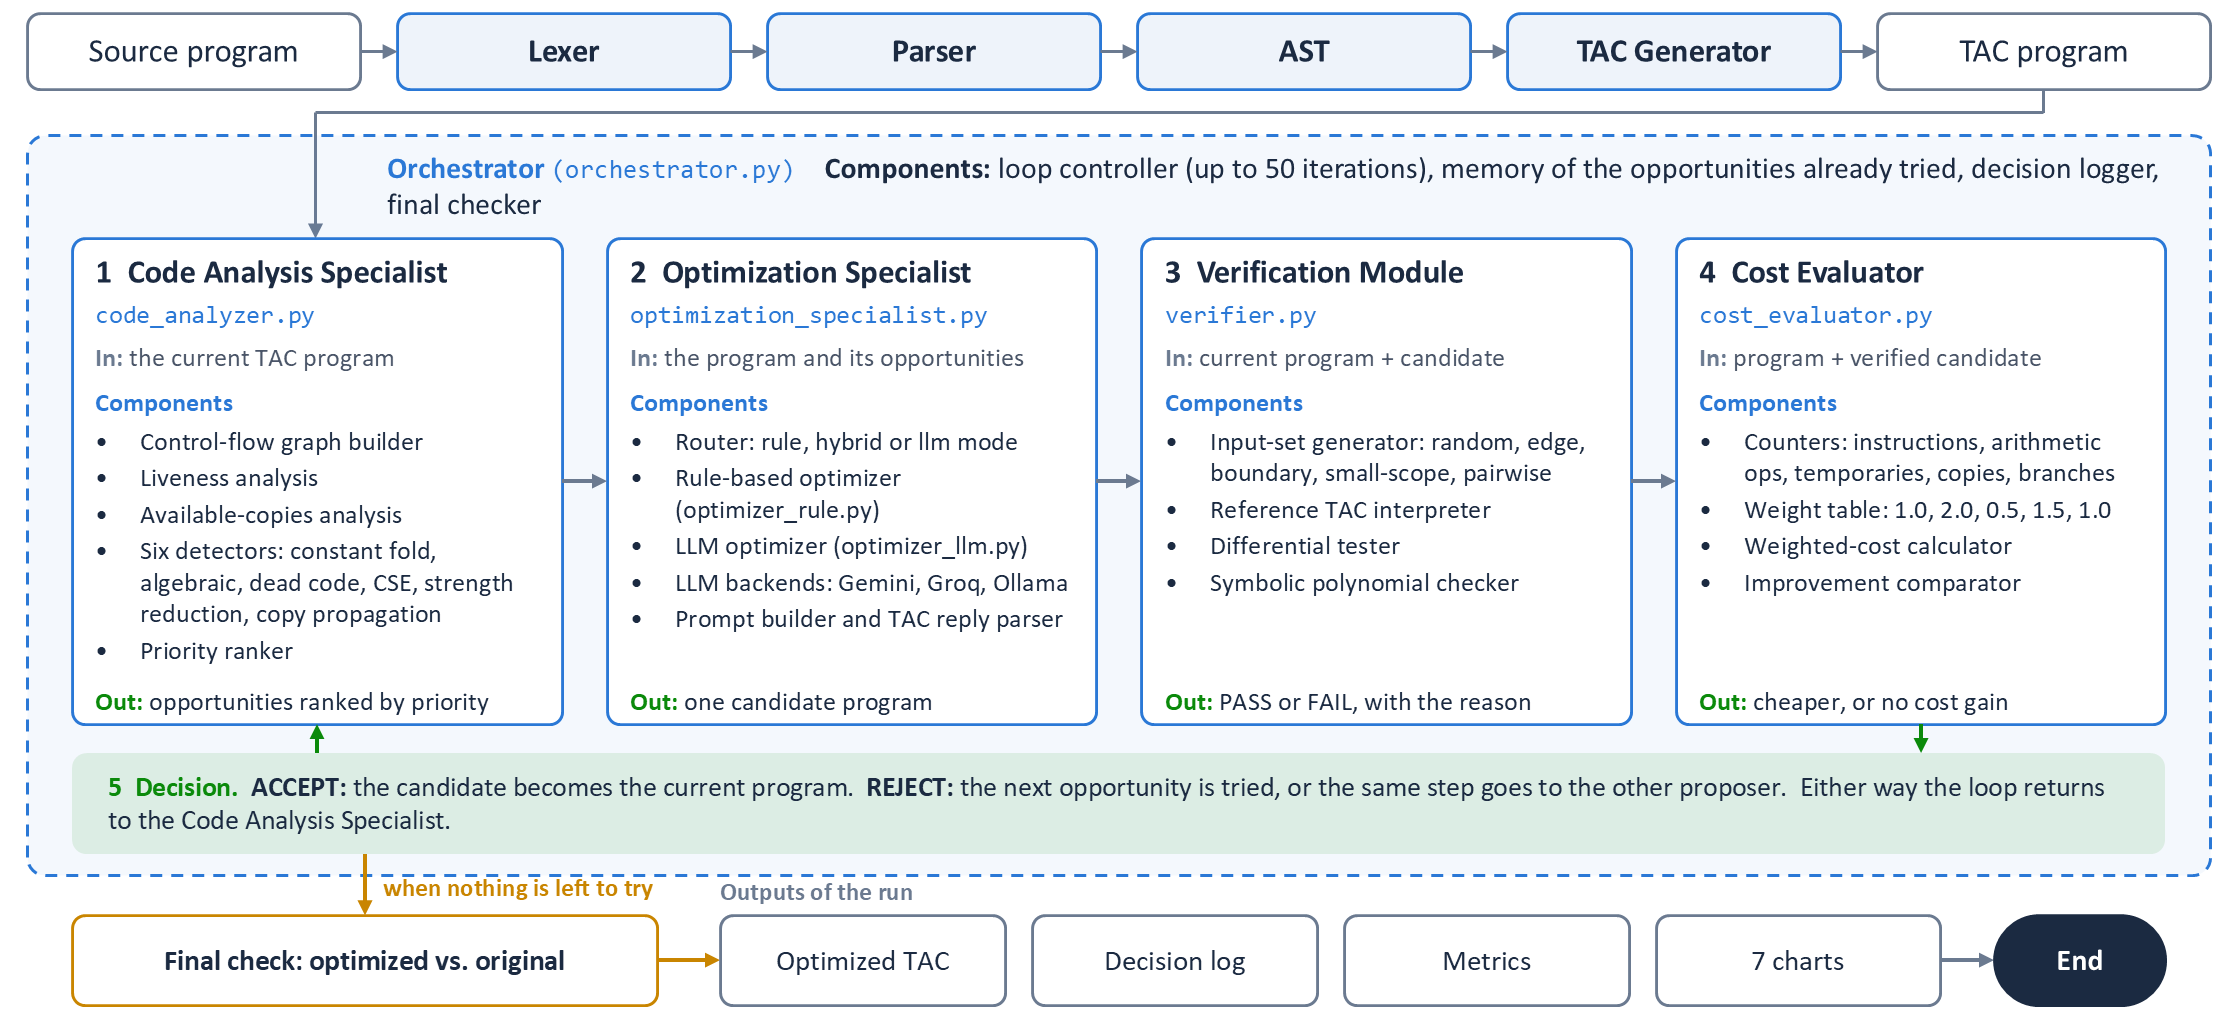
\includegraphics[width=\textwidth]{report_figures/architecture.png}
\caption{System architecture: the frontend, and the agent loop with the work done inside each component.}
\label{fig:architecture}
\end{figure}

\begin{itemize}[leftmargin=2cm]
  \item \textbf{Orchestrator.} Runs the loop for up to 50 iterations per program, remembers which opportunities were already turned down, logs every decision, and re-verifies the final program against the untouched original.
  \item \textbf{Code Analysis Specialist.} Builds the control-flow graph, runs the liveness and available-copies analyses, and returns the opportunities it finds, ranked by priority (constant folding 100, algebraic simplification 90, dead code 80, CSE 70, strength reduction 60, copy propagation 50).
  \item \textbf{Optimization Specialist.} Decides who proposes the next change and returns one candidate program. Option A is the rule-based optimizer, which applies the highest-priority opportunity to a copy of the program. Option B is an LLM, which receives the TAC and is asked for one semantics-preserving optimization.
  \item \textbf{Verification Module.} Runs the current program and the candidate on the same inputs and compares printed output and failure mode; for straight-line code it also checks symbolic equivalence.
  \item \textbf{Cost Evaluator.} Computes the weighted cost of both programs and accepts the change only if the cost strictly drops.
\end{itemize}

\subsection{Routing Between the Rules and the LLM}

The Optimization Specialist has three routing modes, listed in Table~\ref{tab:routing}. Whatever the route, the proposal goes through the same verification and cost gates. The LLM is never asked about a program that is already nothing but constant \texttt{print} instructions, because that form is provably minimal. Every routing decision is written to the decision log together with its reason.

\begin{table}[H]
\centering
\caption{Routing modes of the Optimization Specialist}
\label{tab:routing}
\begin{tabularx}{\textwidth}{|l|l|X|}
\hline
\textbf{Mode} & \textbf{First choice} & \textbf{Falls back to the other proposer when} \\
\hline
\texttt{rule} & Rules & Never: the LLM is not used \\
\hline
\texttt{hybrid} & Rules & The rule proposal for the step was turned down, or the rules have nothing left to try \\
\hline
\texttt{llm} & LLM & The LLM is not running, its call budget is used up, or its proposal was turned down \\
\hline
\end{tabularx}
\end{table}

\subsection{LLM Backends}

All three backends share one prompt and one reply parser, so their results are directly comparable (Table~\ref{tab:backends}). The provider is chosen automatically: Gemini, then Groq, then Ollama, whichever is configured and reachable. An offline switch forces the local model.

\begin{table}[H]
\centering
\caption{The three LLM backends}
\label{tab:backends}
\small
\begin{tabularx}{\textwidth}{|l|l|l|X|}
\hline
\textbf{Backend} & \textbf{Model} & \textbf{Runs on} & \textbf{Notes} \\
\hline
Gemini & \texttt{gemini-3.1-flash-lite} & Google cloud & Free API key; called through the SDK \\
\hline
Groq & \texttt{gpt-oss-120b} & Groq cloud & Free API key; moves to the next model when a daily quota is spent \\
\hline
Ollama & \texttt{qwen2.5-coder:7b} & The laptop & No key and no internet; falls back to the CPU if the GPU runner fails \\
\hline
\end{tabularx}
\end{table}

\subsection{Data Flow Diagram}

\begin{figure}[H]
\centering
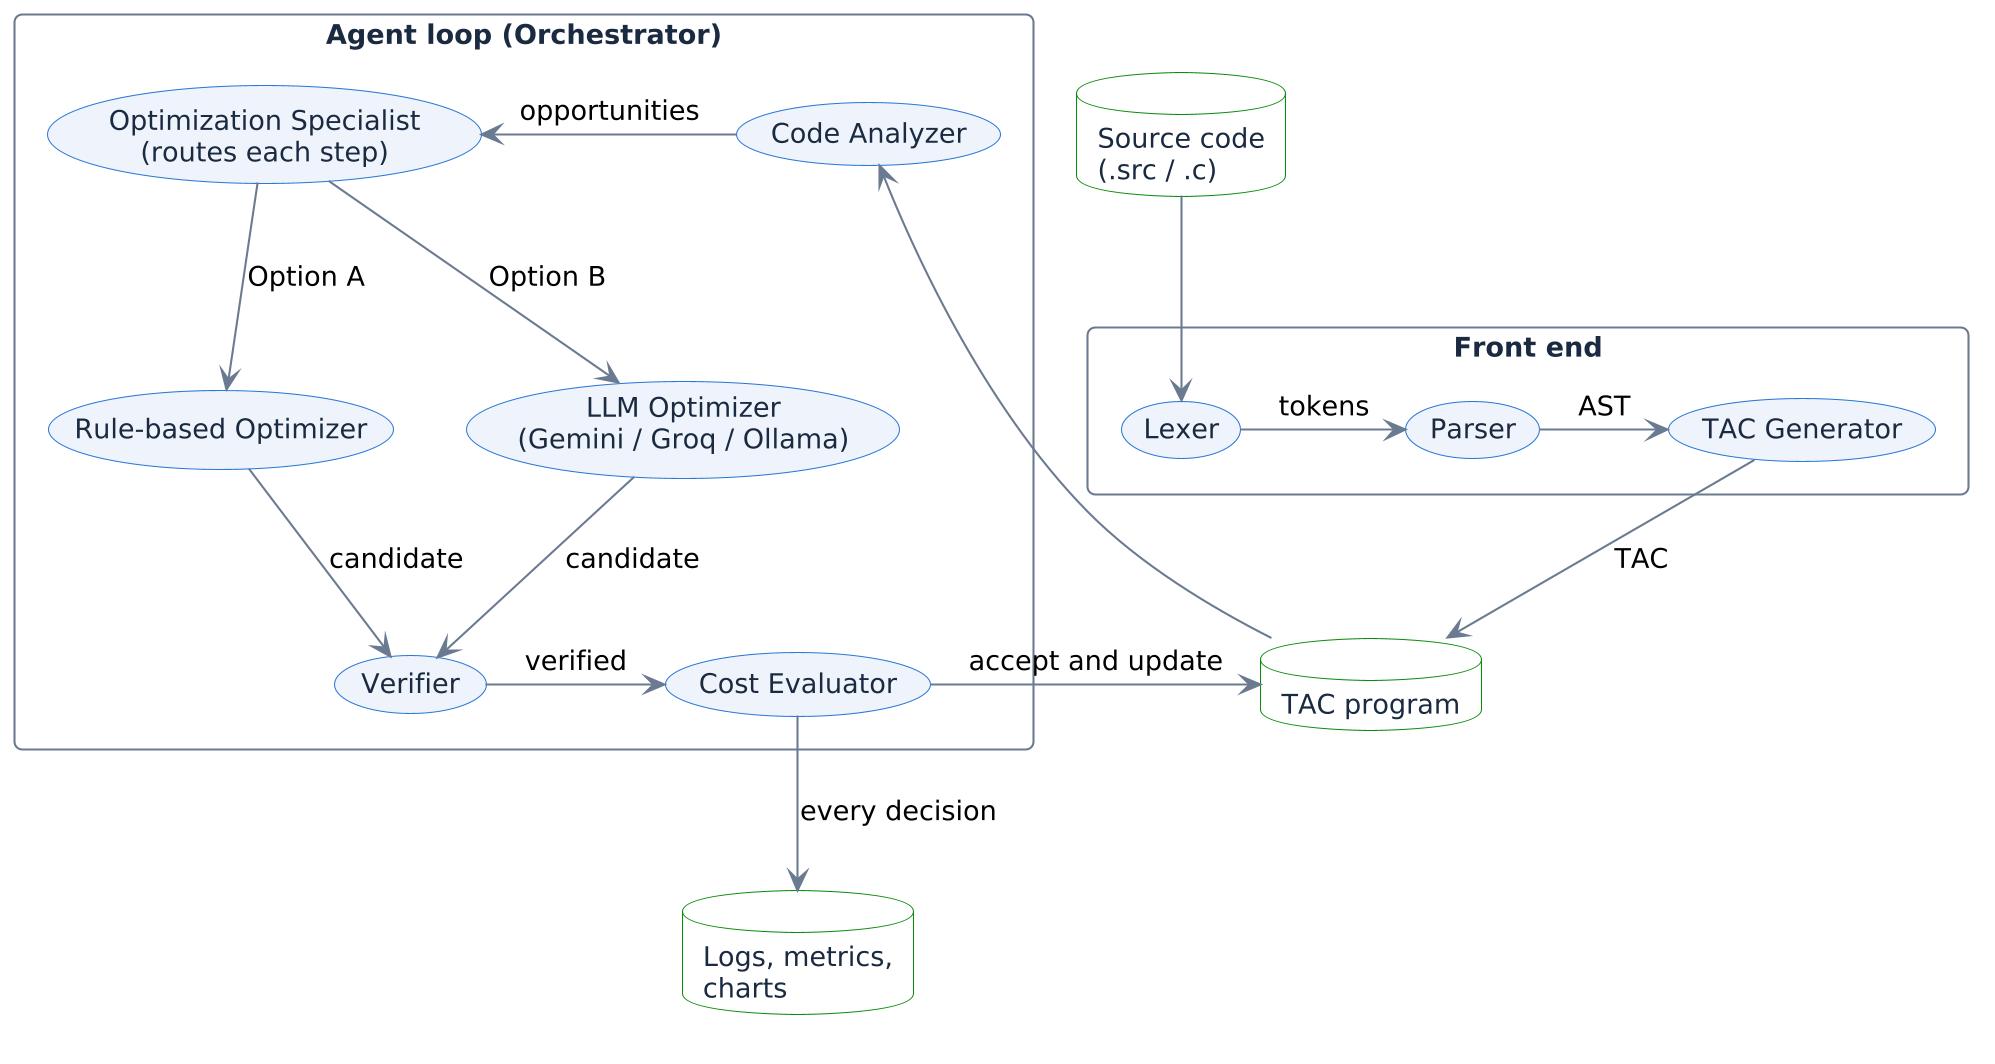
\includegraphics[width=\textwidth]{report_figures/data_flow.png}
\caption{Data flow diagram: source code becomes TAC, each candidate passes the Verifier and the Cost Evaluator, and an accepted change updates the TAC program.}
\end{figure}

\subsection{Class Diagram}

\begin{figure}[H]
\centering
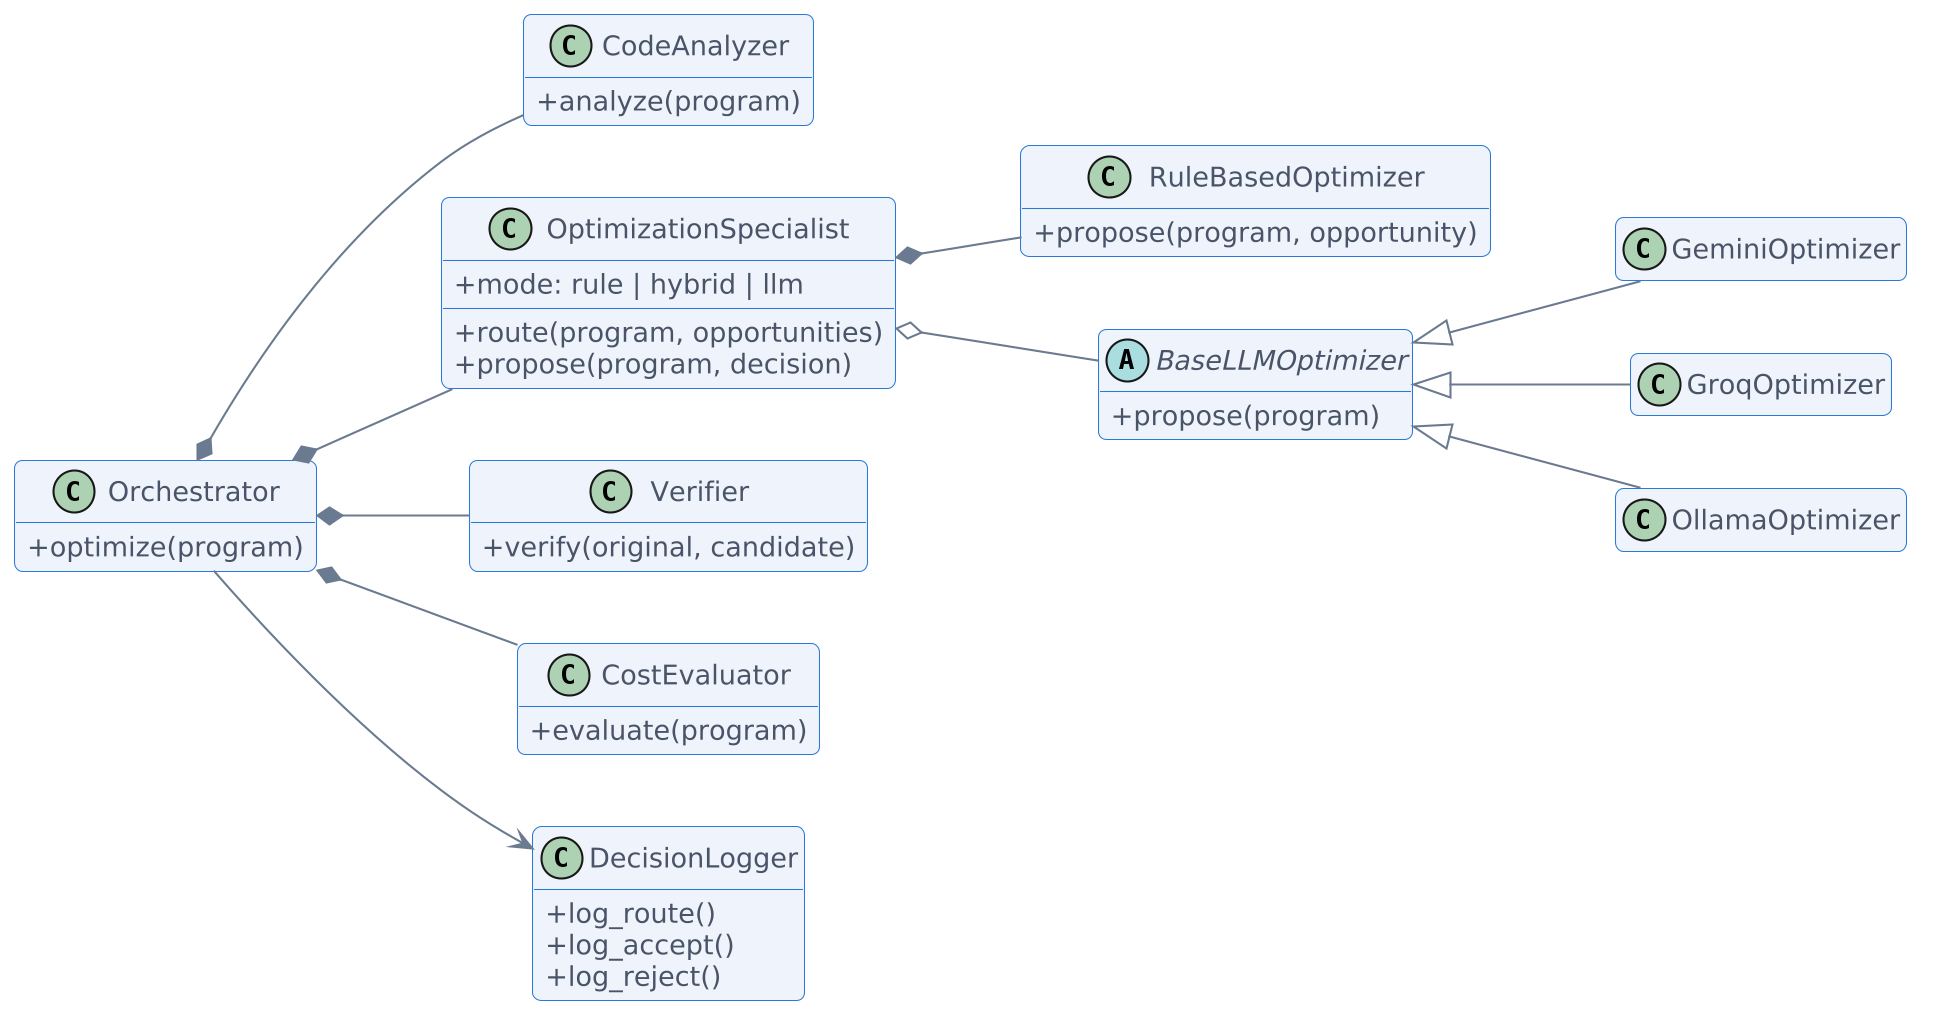
\includegraphics[width=\textwidth]{report_figures/class_diagram.png}
\caption{Class diagram of the agent architecture. The Optimization Specialist owns the rule-based optimizer and holds one of three interchangeable LLM backends.}
\end{figure}

\section{Verification Algorithms}

\textbf{Differential Testing:} The interpreter executes both the original and the candidate TAC on the same input sets. The printed sequence and the failure mode (such as a division by zero or a timeout) must match exactly. The input sets are built in five ways, listed in Table~\ref{tab:inputs}. A program with no inputs has only one possible execution, so for it a match is a proof of equivalence.

\begin{table}[H]
\centering
\caption{Input sets used by differential testing}
\label{tab:inputs}
\begin{tabularx}{\textwidth}{|l|X|l|}
\hline
\textbf{Input sets} & \textbf{What is tried} & \textbf{What it catches} \\
\hline
Random & 20 sets with values from $-100$ to $100$ & General differences \\
\hline
Edge cases & All inputs equal to 0, 1, $-1$, 99, $-99$ & Zero and sign handling \\
\hline
Boundary & $c-1$, $c$, $c+1$ for every literal $c$ & Off-by-one comparisons \\
\hline
Small scope & Every combination of a few small values (one input: every value from $-128$ to $128$) & \texttt{\&\&} against \texttt{||}, a branch on a flag \\
\hline
Pairwise & Every two inputs with every two boundary values & Two inputs that must line up \\
\hline
\end{tabularx}
\end{table}

The last two kinds were added after mutation testing (Section~\ref{sec:testing}) showed that random values almost never make one input zero while another is not, which is exactly what tells \texttt{\&\&} from \texttt{||}.

\textbf{Symbolic Normalization:} For straight-line code, variables are traced as polynomials. $x+x$ and $2 \times x$ normalize to the same multivariate polynomial. If the printed expressions match structurally, the transformation is safe for every input.

\textbf{SMT Verification:} Differential testing shows that two programs agree on the inputs that were tried. For a program with branches but no loops there are finitely many paths, so its whole behaviour can be written as one formula over its inputs. The verifier follows every path symbolically: a branch splits the path in two, and a division splits off the case in which the divisor is zero, where the run stops with what it has printed so far. The paths are then folded into a single description of a run (how it ends, how many values it prints, and the values), and the Z3 solver \citep{demoura2008z3} is asked for an input on which the descriptions of the two programs differ.

\begin{table}[H]
\centering
\caption{The three answers of the SMT stage}
\begin{tabularx}{\textwidth}{|l|X|}
\hline
\textbf{Answer} & \textbf{Meaning and consequence} \\
\hline
\texttt{unsat} & No such input exists: the two programs are equivalent for all inputs. The result is recorded as proved. \\
\hline
\texttt{sat} & Z3 returns the input. It is replayed in the reference interpreter, and if the outputs really differ the proposal is rejected with that counterexample. \\
\hline
\texttt{unknown} & No answer within three seconds, usually because of non-linear arithmetic. The verdict of differential testing stands. \\
\hline
\end{tabularx}
\end{table}

Integers are unbounded and division and modulo follow C, exactly as in the interpreter. The stage runs on every LLM proposal and on the end-to-end check of every program. Programs with loops are outside its scope and remain tested. As an example of what it adds: a program that prints 1 when $3x = 999999$ and 0 otherwise differs from a program that always prints 0 on the single input $x = 333333$, which is near no literal in either program, so every test passes. Z3 finds that input immediately.

\section{Cost Model: Static Cost and Execution Time}
\label{sec:time}

The static cost of a program is a weighted count of its instructions, arithmetic operations, temporaries, copies and branches. It cannot see how often an instruction runs. The Cost Evaluator therefore also measures execution time: the program is run on 25 fixed inputs (20 random sets, half of them positive, and 5 edge cases), every executed instruction adds its latency from Table~\ref{tab:latency}, and the time is the average over the runs. The values given to an input depend only on its name, so a program and a candidate are timed on the same data.

\begin{table}[H]
\centering
\caption{Latency charged per executed instruction (abstract cycles)}
\label{tab:latency}
\begin{tabular}{|l|c|}
\hline
\textbf{Instruction} & \textbf{Cycles} \\
\hline
Copy, load a constant & 1 \\
\hline
Addition, subtraction, shift, comparison, logic & 1 \\
\hline
Multiplication & 3 \\
\hline
Division, modulo & 20 \\
\hline
Unconditional jump & 1 \\
\hline
Conditional branch & 2 \\
\hline
Print & 1 \\
\hline
Label & 0 \\
\hline
\end{tabular}
\end{table}

Two cost models decide what counts as an improvement. Under the \emph{static} model, the default, a change is accepted if the static cost drops; all results on the generated dataset use it. Under the \emph{time} model a change is accepted if the measured time drops, or if the time is equal and the static cost drops. Every run reports both reductions, whichever model decides.

\section{LLM Self-Repair}
\label{sec:repair}

When an LLM answer is rejected, the reason is specific: the verifier has the inputs on which the outputs differ, or the parser has the line that is not valid TAC. The Optimization Specialist sends the model its rejected answer together with that reason and asks once more. The second answer goes through exactly the same verification and cost gates as any other proposal, so self-repair cannot make the system less safe; it can only turn a wasted call into a useful one. By default one repair is allowed per rejected answer, and repairs do not use up the budget of fresh proposals.


% ============================================================
\chapter{IMPLEMENTATION}

\section{Core Modules}

We structured the codebase into distinct modules to keep concerns separated:
\begin{itemize}[leftmargin=2cm]
  \item \texttt{src/frontend/}: Handles lexical analysis and recursive-descent parsing, and lowers AST nodes to TAC instructions. A second front end accepts a subset of real C for the live demo.
  \item \texttt{src/tac/}: Contains the iterative dataflow engines (liveness for DCE, available copies for propagation) and the TAC interpreter used for testing.
  \item \texttt{src/agents/}: Contains the five components. \texttt{orchestrator.py} runs the loop; \texttt{code\_analyzer.py} finds opportunities; \texttt{optimization\_specialist.py} routes each step and owns \texttt{optimizer\_rule.py} and \texttt{optimizer\_llm.py} (Gemini, Groq and Ollama); \texttt{verifier.py} and \texttt{cost\_evaluator.py} are the two gates.
  \item \texttt{src/visualization/}: Produces the metrics report and the seven charts.
\end{itemize}

Below is the core logic driving the Orchestrator. It enforces our safety rules: a change is only kept if it passes verification \emph{and} reduces the static cost score. If the proposal for a step is turned down, the Specialist may hand the same step to the other proposer.

\begin{lstlisting}[language=Python, caption={The Orchestrator loop (trimmed)}, label=lst:orch]
for iteration in range(1, self.max_iterations + 1):
    # 1. ANALYZE (leaving out opportunities already turned down)
    opportunities = [o for o in self.analyzer.analyze(current)
                     if self._opportunity_key(o) not in attempted]

    # 2-5. PROPOSE -> VERIFY -> EVALUATE -> ACCEPT/REJECT
    tried, outcome = [], None
    while outcome not in ("accepted", "unverifiable"):
        decision = specialist.route(current, opportunities,
                                    llm_calls, tried)
        if decision.route is None:
            break                    # nobody can propose anything more
        tried.append(decision.route)
        proposal = specialist.propose(current, decision, opportunities)
        outcome = self._judge(iteration, current, proposal)
        if outcome == "accepted":
            current = proposal.candidate
            attempted.clear()        # new opportunities may appear

    if outcome != "accepted" and not opportunities:
        break                        # converged: nothing left to try
\end{lstlisting}

The routing decision itself is a short method of the Optimization Specialist. The mode sets the order in which the two proposers are considered, and a proposer is skipped when it has nothing to offer.

\begin{lstlisting}[language=Python, caption={The routing decision (trimmed)}, label=lst:route]
def route(self, program, opportunities, llm_calls=0, tried=()):
    order = ([Route.RULE, Route.LLM] if self.mode != "llm"
             else [Route.LLM, Route.RULE])
    if not self.llm_attached:
        order = [Route.RULE]
    passed_over, llm_note = [], ""
    for route in order:
        if route in tried:
            name = "rule-based" if route is Route.RULE else "LLM"
            passed_over.append(f"the {name} proposal was turned down")
        elif route is Route.RULE and not opportunities:
            passed_over.append("the rules have nothing left to try")
        elif route is Route.LLM and (
                llm_note := self._llm_blocker(program, llm_calls)):
            passed_over.append(f"LLM not used, {llm_note}")
        else:
            reason = self._reason(route, opportunities, passed_over)
            return RoutingDecision(route, reason, llm_note)
    return RoutingDecision(None, "; ".join(passed_over), llm_note)
\end{lstlisting}

\section{Testing Strategy}
\label{sec:testing}

We validated the implementation with a suite of 397 automated tests covering every module. The LLM backends are tested against stand-in local servers, so the tests need no API key, no Ollama installation and no network.

To test the verifier itself, we first injected hand-written broken optimizations (swapping subtraction operands, dropping live stores, introducing off-by-one loop conditions) and checked that each one was rejected. We then tested the system at a larger scale:

\begin{itemize}[leftmargin=2cm]
  \item \textbf{Fuzzing the rules.} 5,100 random TAC programs were generated, and all 20,968 rule-based proposals for them were compared with the original on inputs the verifier does not use. None changed the program's behaviour.
  \item \textbf{Mutation testing the verifier.} Random branching programs were changed in one place (an operator, a constant or an operand), the way a wrong LLM proposal might be. Of the first 400 mutants, the verifier accepted 194, and 13 of those behaved differently from the original. After the small-scope and pairwise input sets were added, the verifier accepted 351 of 800 mutants and none of them behaves differently.
  \item \textbf{Re-checking the results.} For every run, each final program was executed against its original on every combination of small input values plus random ones (about 64,000 executions per run). No mismatch was found.
  \item \textbf{Replaying the Gemini run.} The 383 recorded Gemini replies were replayed through the strengthened verifier. Every proposal received the same decision as before.
\end{itemize}

The same testing found one bug in the rules: strength reduction rewrote $x \times 2^k$ to a shift even for $k > 64$, which the interpreter rejects. The proposal was caught by the verifier every time, and the analyzer no longer makes it.

The additions for the final review are tested in the same way. The SMT stage is checked against hand-built pairs of programs: equivalent ones must be proved, and pairs that differ on a single input, in the order of their output, or in whether a division traps must be refuted with the right counterexample.

\textbf{Re-checking the runs on real programs.} Every optimized program was run against its original on inputs the verifier had not used, including values up to a million. For the two rule-based runs and the local-model run no mismatch was found. In the Groq run the re-check found one wrong program. The model had replaced \texttt{x - 1} by the constant 9 inside a loop in which \texttt{x} is multiplied by ten in every iteration. The change is correct while \texttt{x} is 10, and the loop runs a second time only for inputs of 100 or more, which none of the verifier's input sets reached, so all 388 tests had passed. The verifier now adds 60 wide-range input sets for every program that reads input: values up to a thousand, ten thousand, a million and a billion, signed values, and powers of ten with their neighbours. A run that is too long for these inputs is skipped, so they never make a program unverifiable. With them the wrong change is rejected with a counterexample. The affected program was optimized again, and the re-check of all runs on real programs (258,912 executions) now finds 0 mismatches. The four runs on the generated dataset were re-checked on the same wide inputs, also without a mismatch.


% ============================================================
\chapter{RESULTS AND DISCUSSION}

\section{Optimization Performance}

We ran four passes over the 500 programs: a baseline using only the rule-based optimizer, and three \texttt{hybrid} runs in which an LLM is asked when the rules hit a wall. Table~\ref{tab:metrics} gives the key metrics.

\begin{table}[H]
\centering
\caption{Key metrics from the four 500-program runs}
\label{tab:metrics}
\small
\begin{tabular}{lcccc}
\toprule
\textbf{Metric} & \textbf{Rule-Only} & \textbf{+ Gemini} & \textbf{+ Groq} & \textbf{+ Ollama} \\
\midrule
Avg. cost reduction & 82.49\% & 91.50\% & 90.89\% & 83.28\% \\
Total proposals & 10,628 & 10,978 & 11,085 & 10,805 \\
Accepted & 10,517 & 10,828 & 10,925 & 10,579 \\
Verification pass rate & 100.00\% & 99.76\% & 99.95\% & 98.95\% \\
Acceptance rate (of verified) & 98.96\% & 98.87\% & 98.61\% & 98.94\% \\
Steps to convergence (mean) & 22.2 & 22.7 & 22.9 & 22.3 \\
LLM validity rate & --- & 92.35\% & 98.11\% & 42.93\% \\
False positives (silent bugs) & \textbf{0} & \textbf{0} & \textbf{0} & \textbf{0} \\
\bottomrule
\end{tabular}
\end{table}

The rules handled arithmetic and dead code perfectly. The LLMs' main contribution was in loops and conditionals. A rule engine cannot collapse a loop into a single constant, but an LLM can work out the result of a constant loop and replace it. Table~\ref{tab:categories} breaks down the cost reduction by program category.

\begin{table}[H]
\centering
\caption{Per-category cost reduction}
\label{tab:categories}
\small
\begin{tabular}{|l|c|c|c|c|c|}
\hline
\textbf{Category} & \textbf{Programs} & \textbf{Rule-only} & \textbf{+ Gemini} & \textbf{+ Groq} & \textbf{+ Ollama} \\
\hline
Arithmetic & 60 & 96.03\% & 96.03\% & 96.03\% & 96.03\% \\
Nested & 60 & 98.10\% & 98.22\% & 98.31\% & 98.19\% \\
Repeated expr & 60 & 80.71\% & 81.65\% & 80.94\% & 80.71\% \\
Dead code & 60 & 97.44\% & 97.44\% & 97.44\% & 97.44\% \\
\textbf{Loops} & \textbf{80} & \textbf{65.05\%} & \textbf{93.35\%} & \textbf{93.43\%} & \textbf{66.09\%} \\
\textbf{Conditionals} & \textbf{80} & \textbf{73.91\%} & \textbf{84.07\%} & \textbf{83.48\%} & \textbf{75.21\%} \\
\textbf{Mixed} & \textbf{100} & \textbf{77.91\%} & \textbf{91.56\%} & \textbf{89.29\%} & \textbf{79.96\%} \\
\hline
\textbf{All} & \textbf{500} & \textbf{82.49\%} & \textbf{91.50\%} & \textbf{90.89\%} & \textbf{83.28\%} \\
\hline
\end{tabular}
\end{table}

\section{Comparing the Three LLMs}

Table~\ref{tab:llms} compares what each model contributed. No run made any program worse than the rule-only baseline.

\begin{table}[H]
\centering
\caption{The three LLMs on the same 500 programs}
\label{tab:llms}
\small
\begin{tabular}{lccc}
\toprule
 & \textbf{Gemini} & \textbf{Groq} & \textbf{Ollama} \\
\midrule
Runs on & Google cloud & Groq cloud & Laptop (CPU) \\
Programs improved over rules & 196 & 181 & 32 \\
Calls to the model & 383 & 359 & 328 \\
Usable proposals & 340 & 318 & 198 \\
\quad accepted & 262 & 248 & 60 \\
\quad correct, but no cheaper & 52 & 64 & 25 \\
\quad wrong, blocked by the verifier & 26 & 6 & 113 \\
Validity rate & 92.35\% & 98.11\% & 42.93\% \\
Time for the full run & 43 min & 42 min & 2 h 14 min \\
\bottomrule
\end{tabular}
\end{table}

Gemini and Groq reach almost the same result. Groq's models were the most reliable: only 6 of 318 proposals were wrong. During the Groq run the first model (\texttt{gpt-oss-120b}) used up its free daily quota after 286 calls, and the system moved on to \texttt{gpt-oss-20b} for the last 148 programs without stopping. The local model was wrong more often than it was right, but because every proposal is verified this cost time and not correctness, and it still improved 32 programs with no internet connection at all.

\section{Sample Run}

Listing~\ref{lst:demo} shows the agent working on a small C program whose loop adds the same constant ten times. The rules clean up the temporaries and fold the constant; when they have nothing left to try, the step is routed to the LLM, which replaces the loop. The whole program becomes one instruction.

\begin{lstlisting}[caption={A real run of the demo on a C loop, with Groq as the LLM (shortened)}, label=lst:demo]
int sum = 0;
for (int i = 0; i < 10; i++) {
    int step = 2 + 3;
    sum += step * 1;
}
printf("%d\n", sum);

22 TAC instructions, weighted cost 56.0

[ 1] COPY_PROPAGATION  t0 = 0 -> uses of t0 -> 0
       verified  cost 56.0 -> 53.0  ACCEPTED
[ 6] CONSTANT_FOLD     t6 = 2 + 3 -> t6 = 5
       verified  cost 41.0 -> 40.5  ACCEPTED
...
[14] COPY_PROPAGATION  t11 = i + 1; i = t11 -> i = i + 1
       verified  cost 22.5 -> 19.5  ACCEPTED
     route to LLM optimizer: the rules have nothing left to try
[15] LLM (Groq)  the loop adds a constant 5 exactly ten times,
     so replace it with sum = 50 and eliminate the dead loop
       verified  cost 19.5 -> 3.5   ACCEPTED
[16] COPY_PROPAGATION  sum = 50 -> uses of sum -> 50
       verified  cost 3.5 -> 1.0    ACCEPTED

Optimized TAC:  print 50        cost 56.0 -> 1.0  (98.2% reduction)
original prints [50], optimized prints [50]: identical output
\end{lstlisting}

\section{Visualizations}

Figures~\ref{fig:sankey} to \ref{fig:heatmap} are drawn from the Gemini run. Figures~\ref{fig:cmp-gemini} to \ref{fig:cmp-ollama} compare each LLM run with the rule-only baseline.

\begin{figure}[H]
\centering
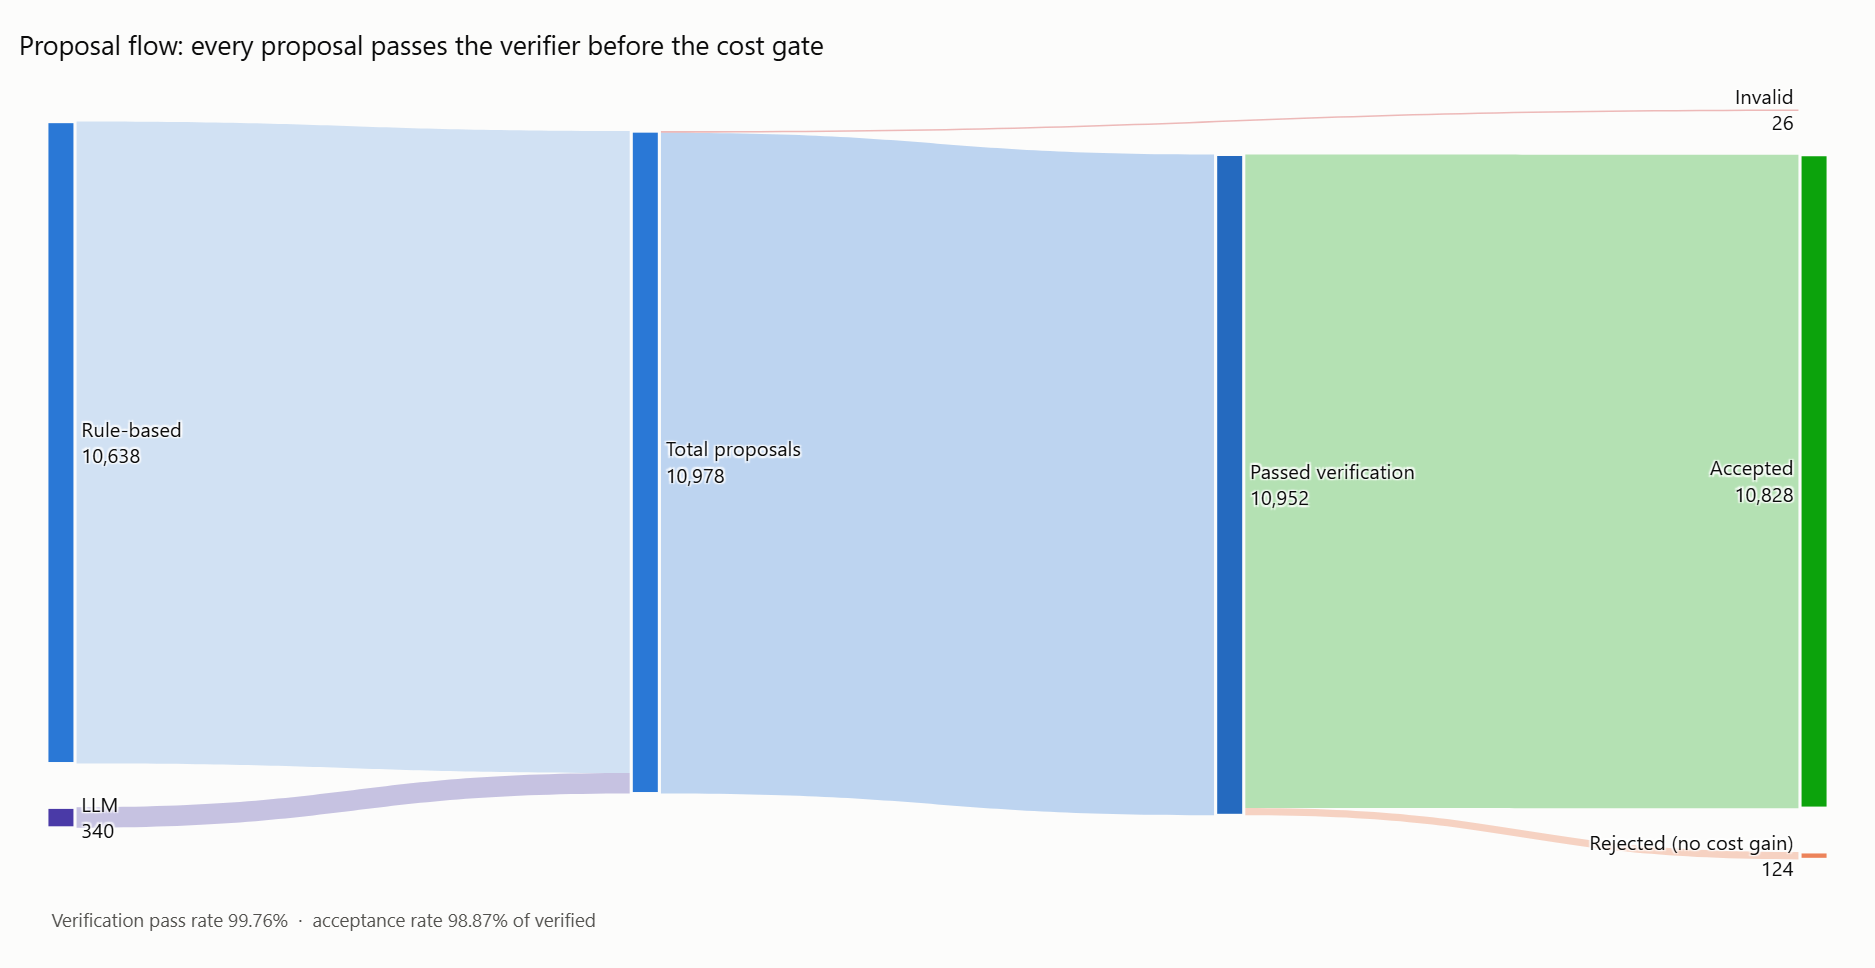
\includegraphics[width=\textwidth]{report_figures/sankey_gemini.png}
\caption{Sankey diagram of the flow of the 10,978 proposals in the Gemini run. The small band at the top is the 26 invalid LLM proposals blocked by the verifier.}
\label{fig:sankey}
\end{figure}

\begin{figure}[H]
\centering
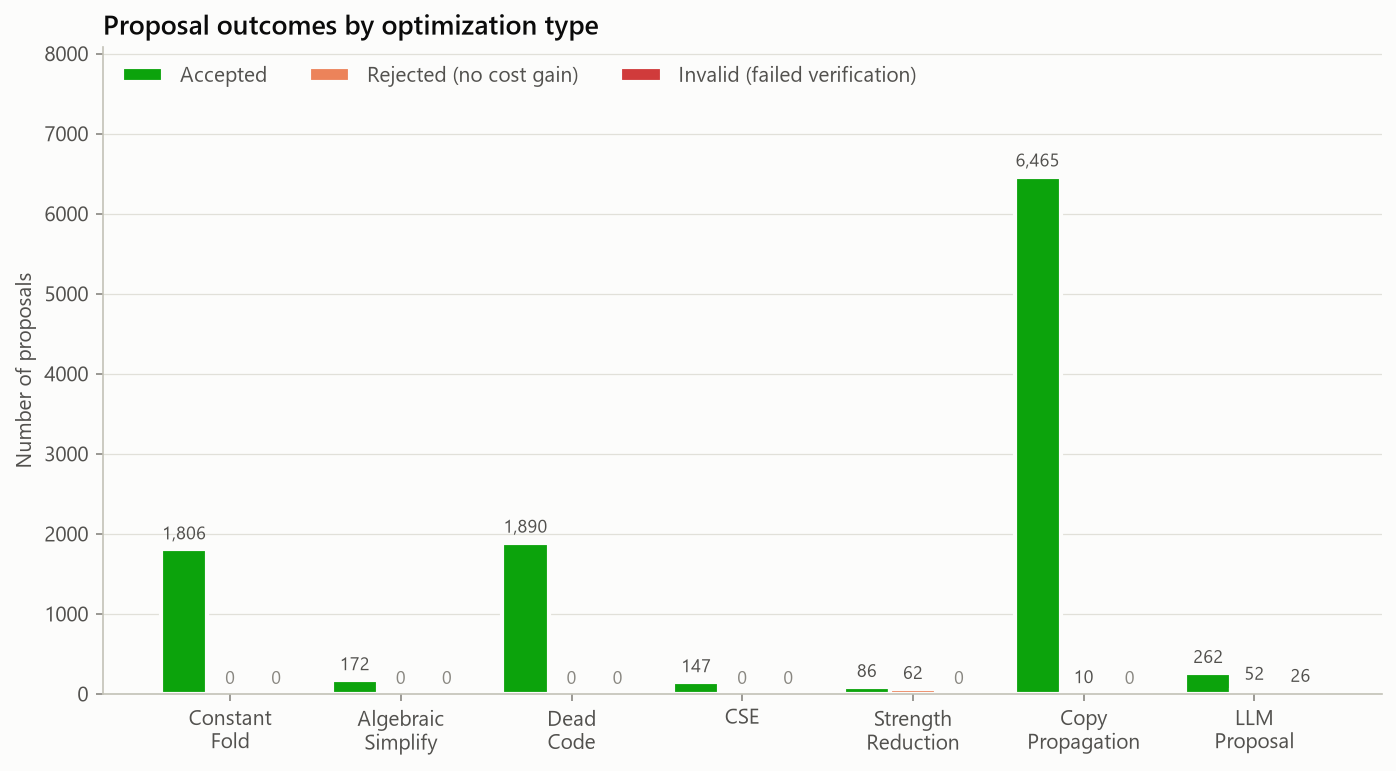
\includegraphics[width=\textwidth]{report_figures/outcomes_by_type_gemini.png}
\caption{Accept, reject, and invalid counts for each optimization type.}
\end{figure}

\begin{figure}[H]
\centering
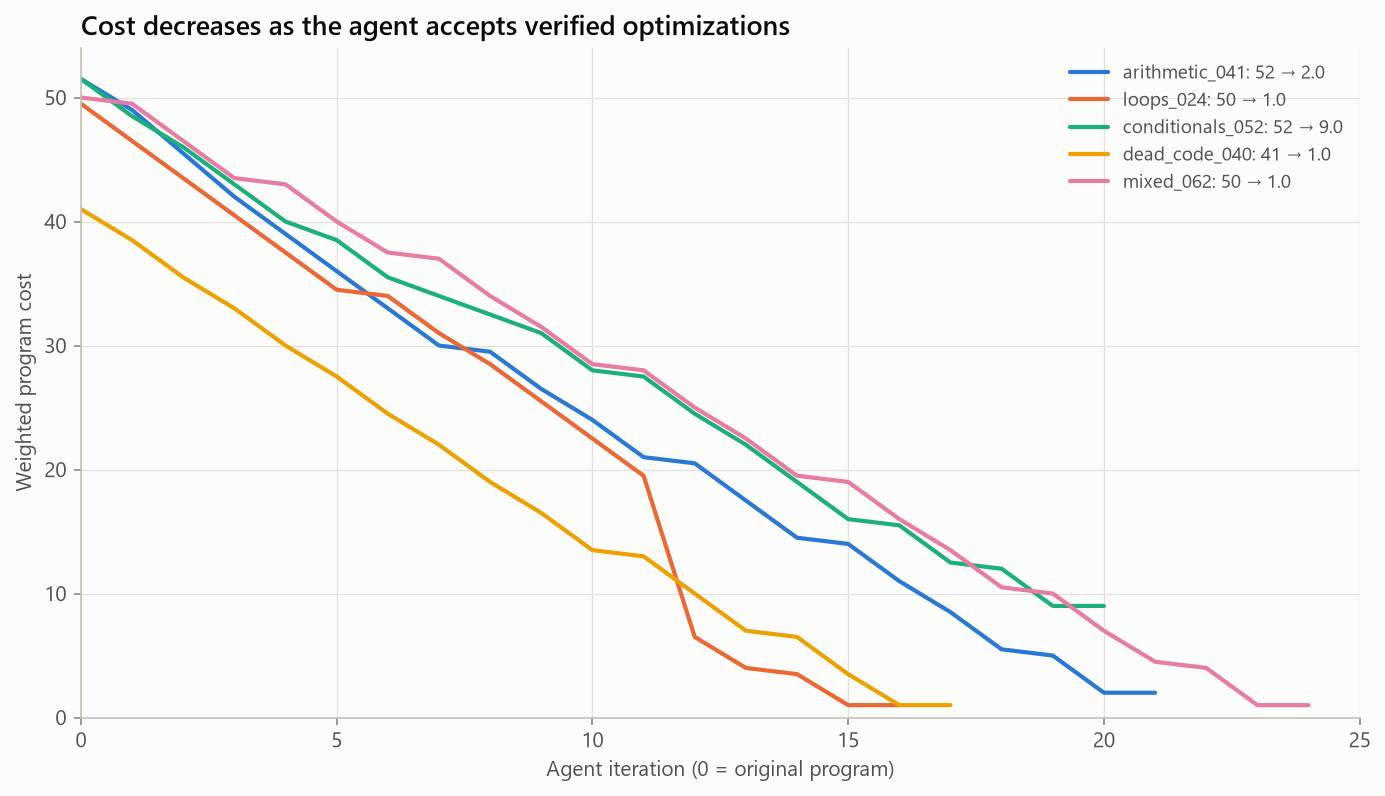
\includegraphics[width=\textwidth]{report_figures/cost_over_iterations_gemini.png}
\caption{Weighted cost over iterations for five representative programs.}
\end{figure}

\begin{figure}[H]
\centering
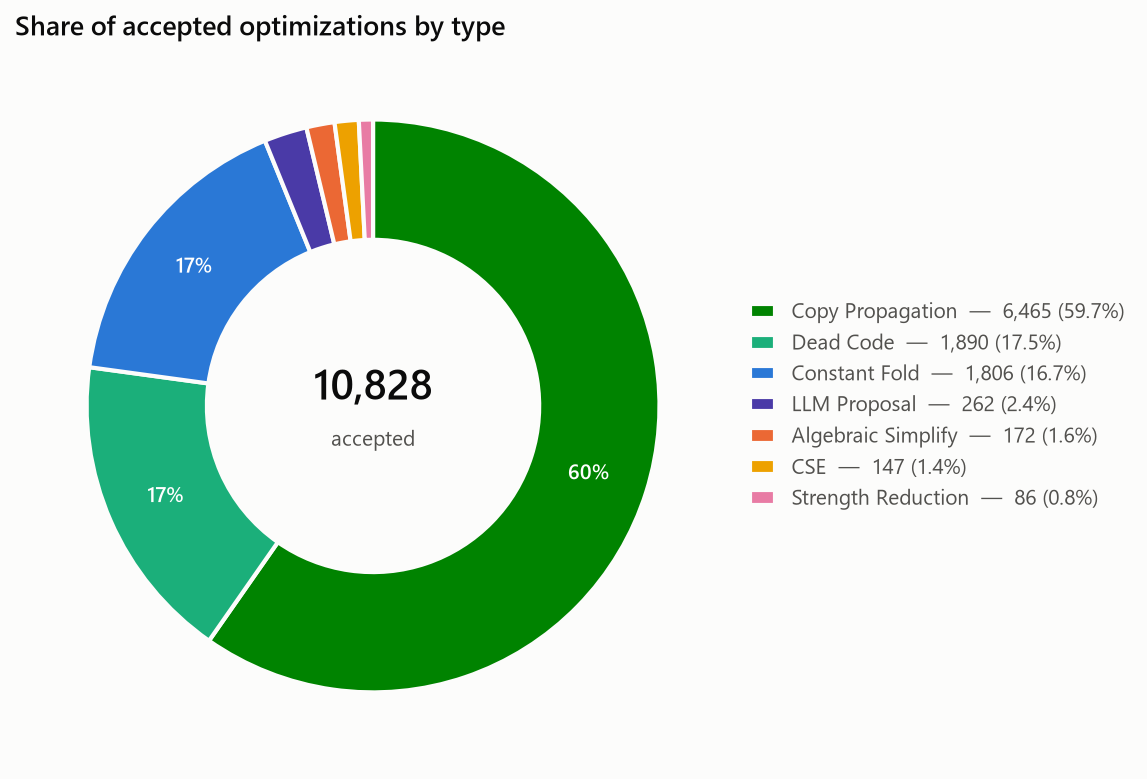
\includegraphics[width=0.9\textwidth]{report_figures/accepted_types_gemini.png}
\caption{Distribution of accepted optimizations. Copy propagation was the most frequent, cleaning up redundant assignments left by other passes.}
\end{figure}

\begin{figure}[H]
\centering
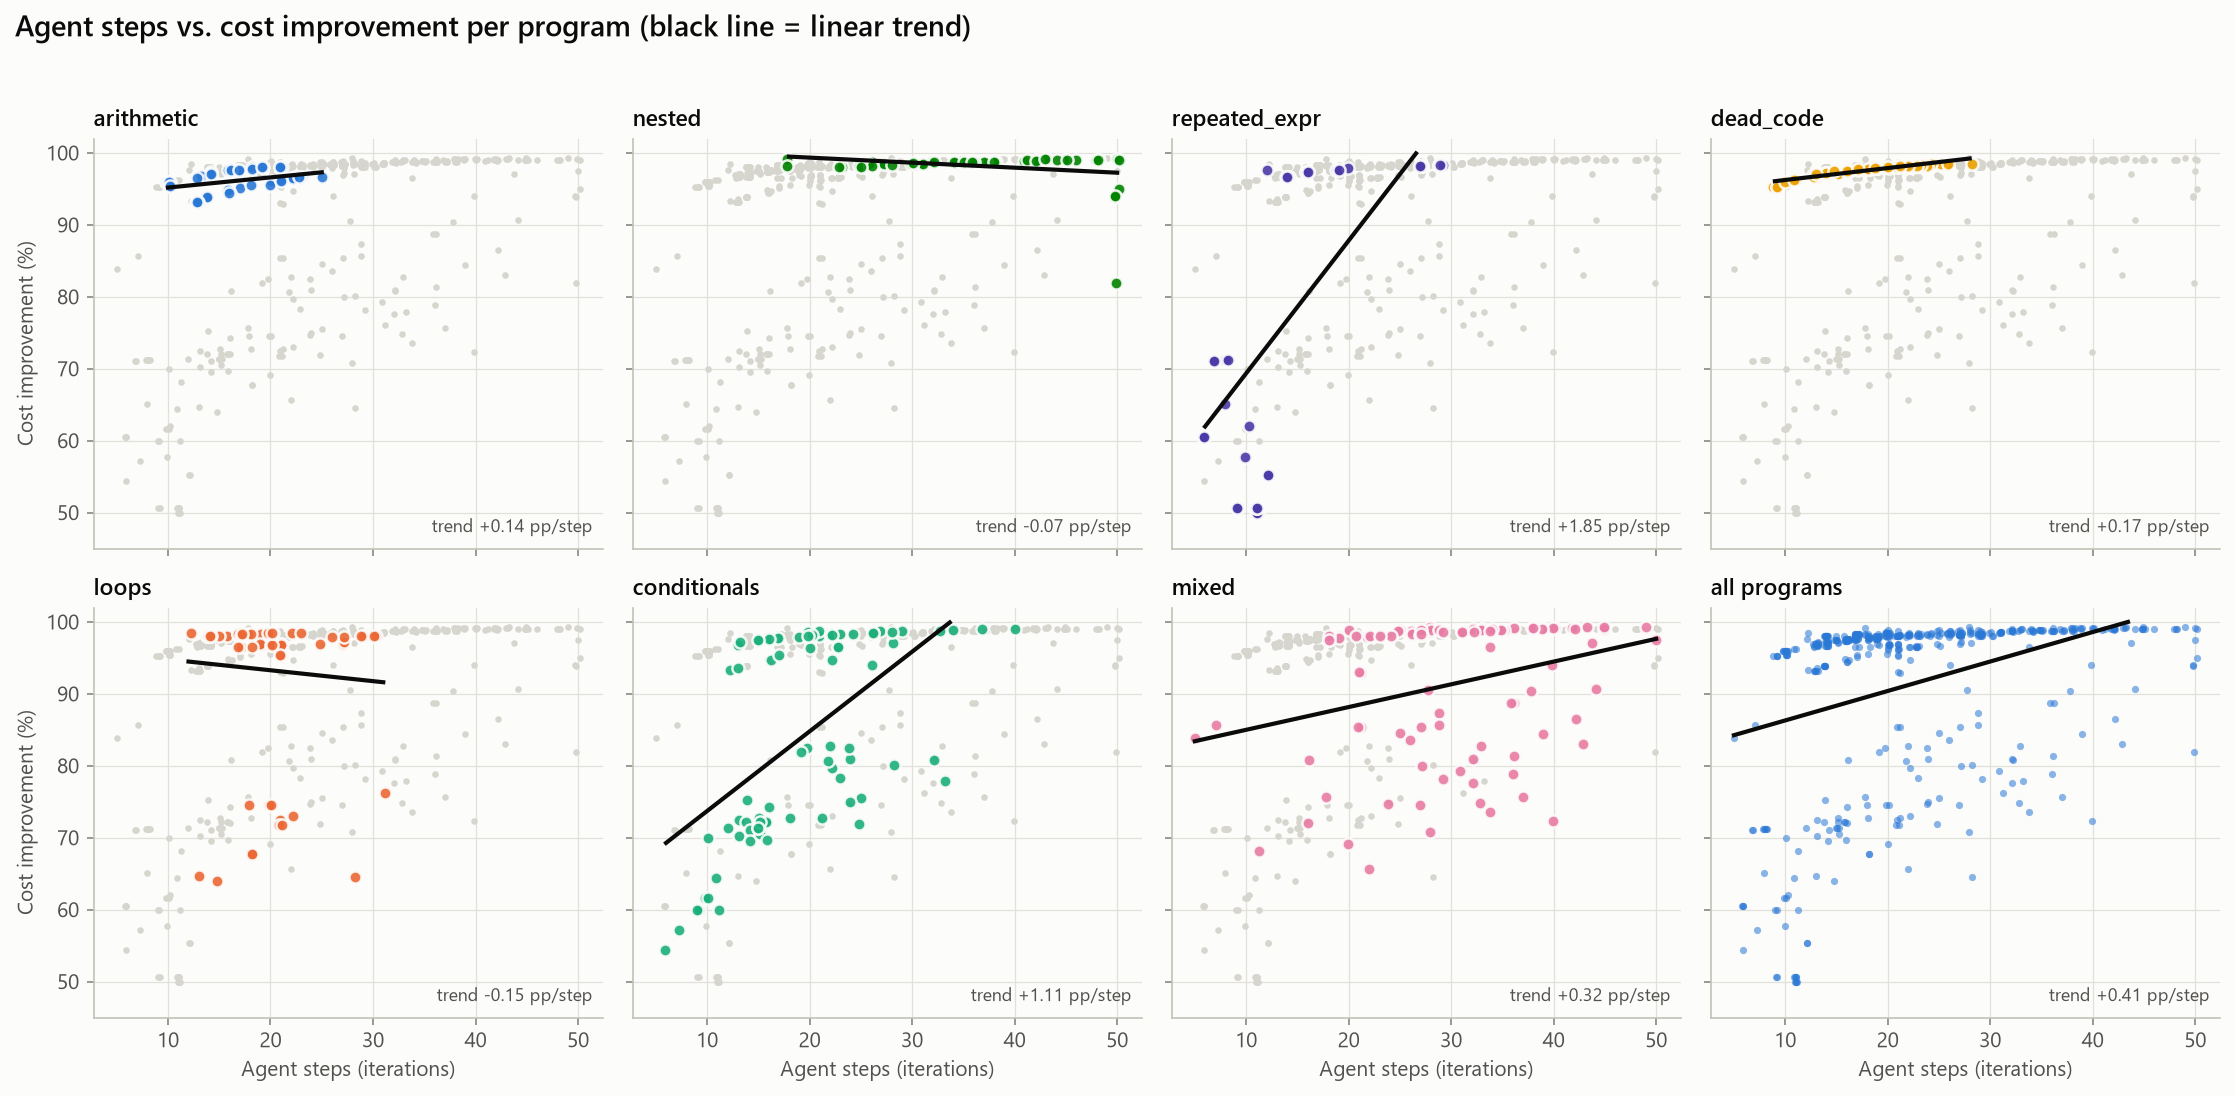
\includegraphics[width=\textwidth]{report_figures/steps_vs_improvement_gemini.png}
\caption{Agent steps taken versus percentage cost improvement, per category.}
\end{figure}

\begin{figure}[H]
\centering
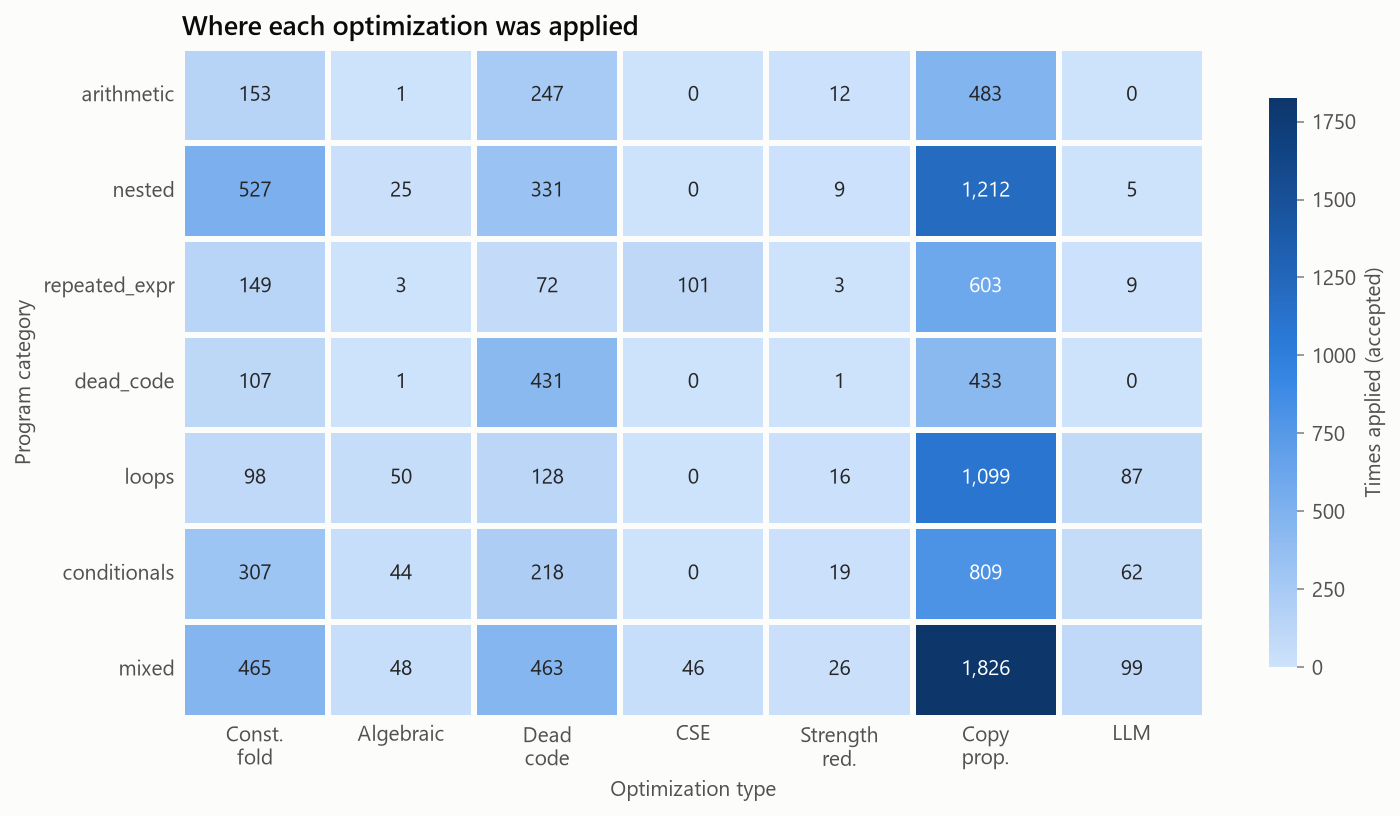
\includegraphics[width=\textwidth]{report_figures/heatmap_gemini.png}
\caption{Heatmap of accepted optimizations, showing which categories benefited most from which optimization.}
\label{fig:heatmap}
\end{figure}

\begin{figure}[H]
\centering
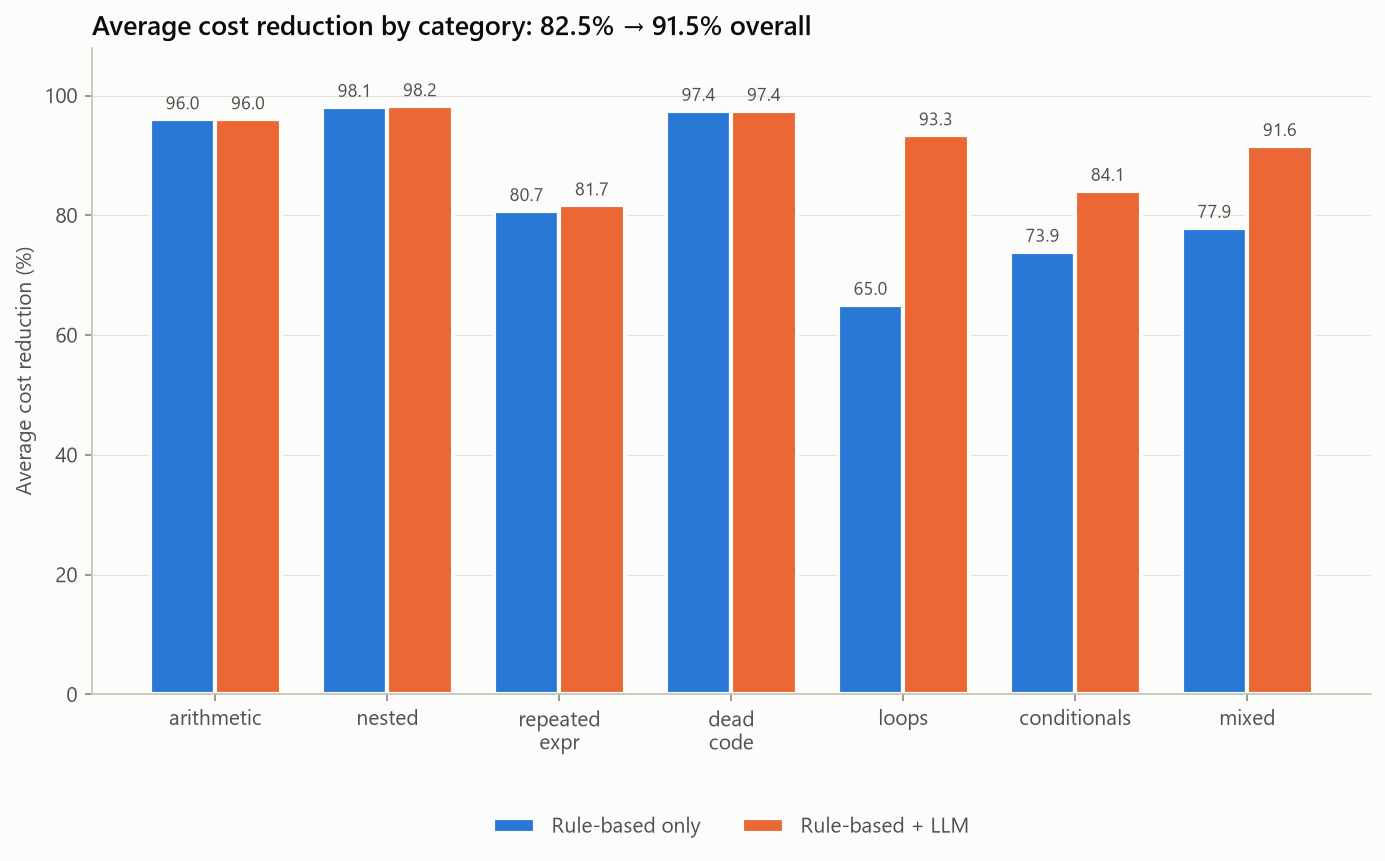
\includegraphics[width=0.9\textwidth]{report_figures/comparison_gemini.png}
\caption{Rule-only against rules + Gemini. Loops rise from 65\% to 93\%.}
\label{fig:cmp-gemini}
\end{figure}

\begin{figure}[H]
\centering
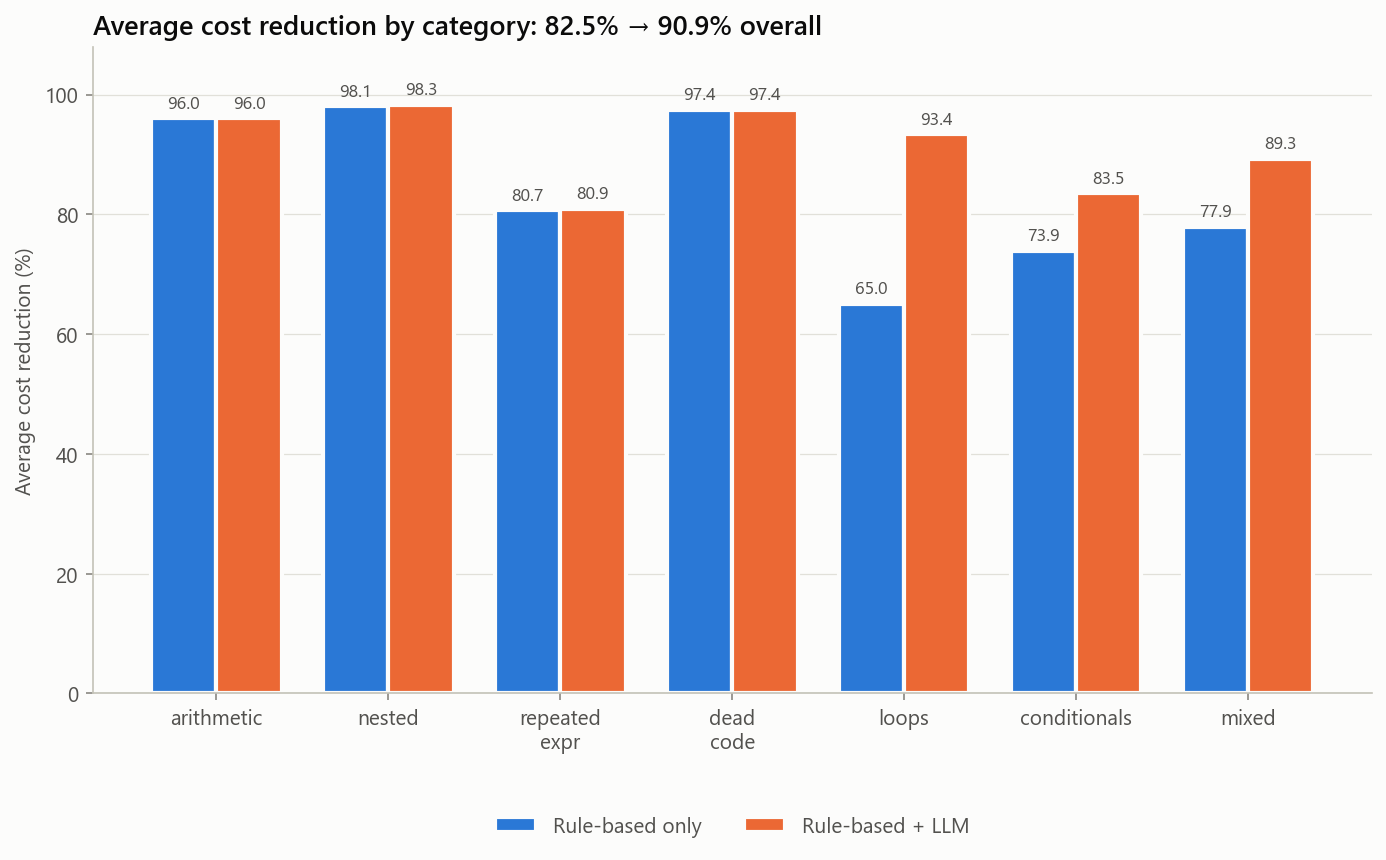
\includegraphics[width=0.9\textwidth]{report_figures/comparison_groq.png}
\caption{Rule-only against rules + Groq. The pattern is the same as with Gemini.}
\end{figure}

\begin{figure}[H]
\centering
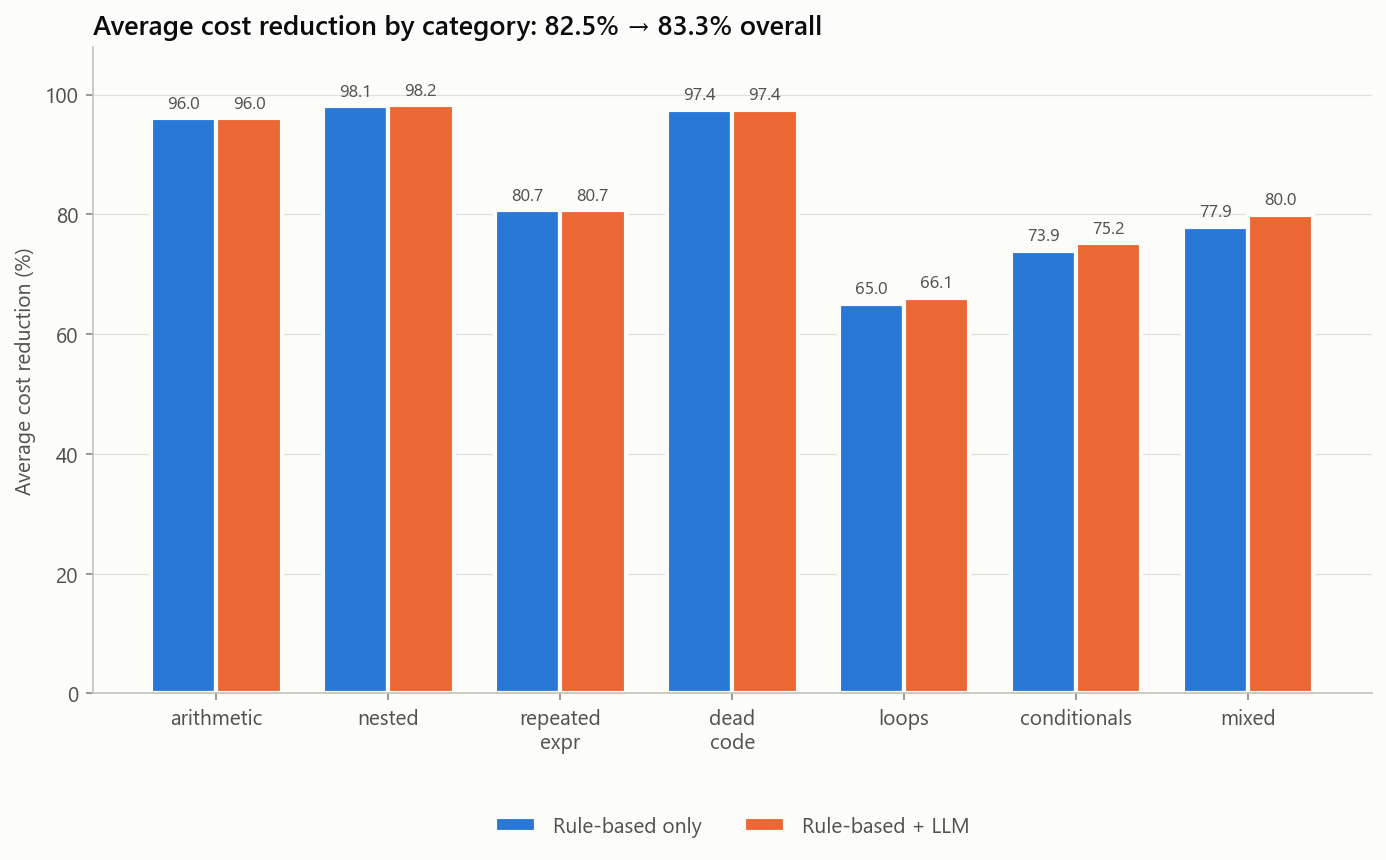
\includegraphics[width=0.9\textwidth]{report_figures/comparison_ollama.png}
\caption{Rule-only against rules + the local Ollama model. The gains are small but come with no internet connection.}
\label{fig:cmp-ollama}
\end{figure}

\section{Results on Real Programs}
\label{sec:realresults}

All runs in this section use the real-program dataset of Section~\ref{sec:realdata} and allow 200 iterations per program, because real programs are longer than the generated ones.

\subsection{Rule-Based Optimization}

\begin{table}[H]
\centering
\caption{Rules only: generated and real programs (static cost model)}
\begin{tabular}{|l|c|c|c|c|c|}
\hline
\textbf{Category} & \textbf{Programs} & \textbf{Generated} & \textbf{Real} & \textbf{Real, time} & \textbf{Proved} \\
\hline
Arithmetic-only & 60 & 96.03\% & 63.26\% & 21.84\% & 60 \\
\hline
Nested expressions & 60 & 98.10\% & 51.62\% & 20.89\% & 60 \\
\hline
Repeated expressions & 60 & 80.71\% & 47.08\% & 25.59\% & 25 \\
\hline
Dead code & 60 & 97.44\% & 56.12\% & 32.08\% & 29 \\
\hline
Loops & 80 & 65.05\% & 49.40\% & 22.69\% & 0 \\
\hline
Conditionals & 80 & 73.91\% & 53.12\% & 32.31\% & 79 \\
\hline
Mixed & 100 & 77.91\% & 48.75\% & 21.71\% & 0 \\
\hline
\textbf{All} & 500 & 82.49\% & \textbf{52.32\%} & 25.19\% & 253 \\
\hline
\end{tabular}
\end{table}

On the real programs the rules reduce the static cost by 52.32\% on average (median 51.88\%); 495 of the 500 programs improve by more than 30\%. The figure is lower than on the generated set because nearly all real programs read their values with \texttt{scanf}, so nothing folds down to a constant. Most of what the rules remove is the redundancy of the naive TAC translation: 6,457 accepted copy propagations and 1,757 dead-code removals, against 143 common subexpressions and 41 constant folds. All 10,546 proposals passed verification; 8,450 were accepted and 2,096 gave no cost gain.

\begin{figure}[H]
\centering
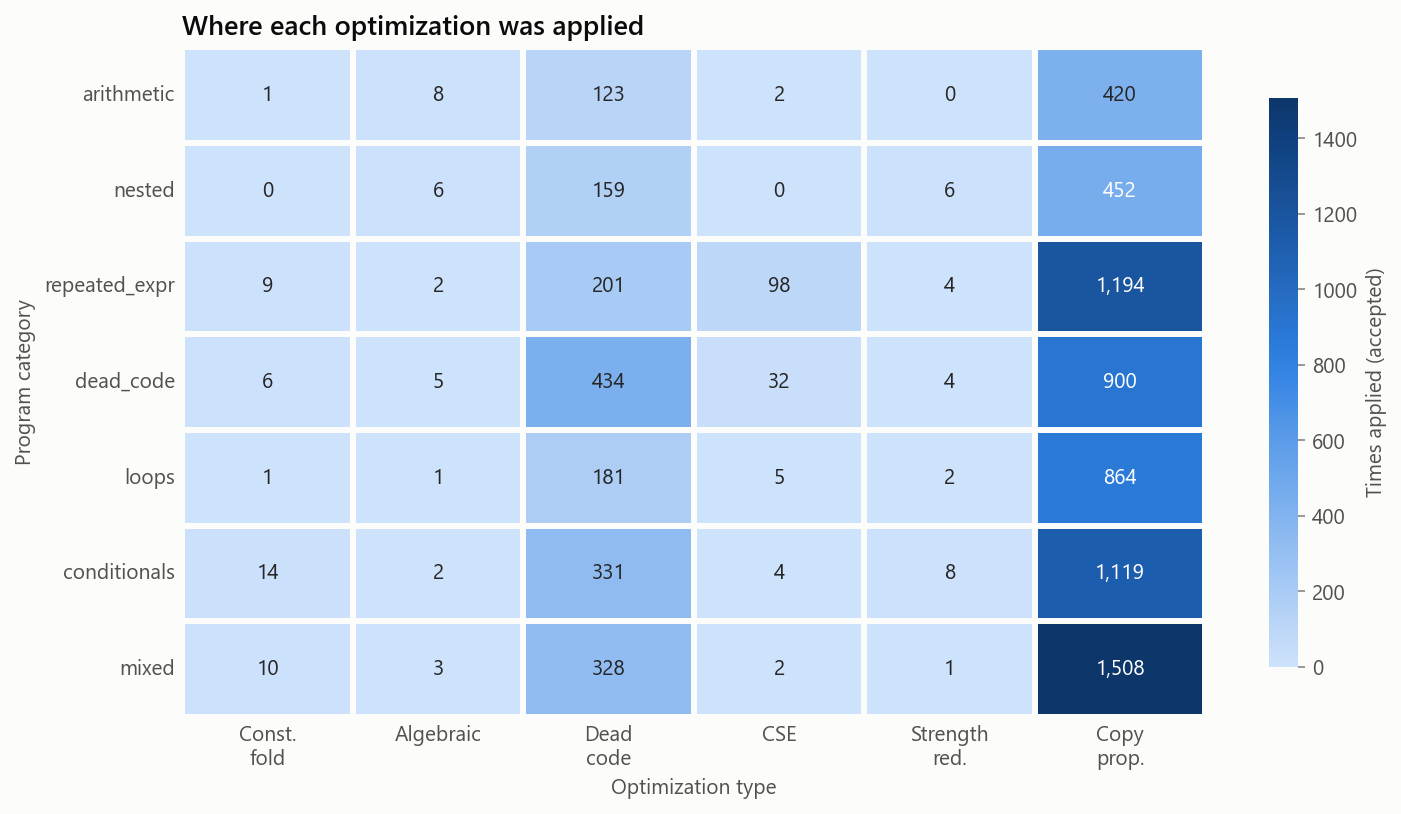
\includegraphics[width=\textwidth]{report_figures/real_heatmap_rules.png}
\caption{Real programs, rules only: accepted optimizations by category and type}
\end{figure}

\subsection{Execution Time and the Two Cost Models}

\begin{table}[H]
\centering
\caption{Rules only on the 500 real programs under the two cost models}
\begin{tabular}{|l|c|c|}
\hline
\textbf{Metric} & \textbf{Static model} & \textbf{Time model} \\
\hline
Average static cost reduction & 52.32\% & 52.32\% \\
\hline
Average execution-time reduction & 25.19\% & 26.45\% \\
\hline
Median execution-time reduction & 21.44\% & 21.96\% \\
\hline
Strength reductions accepted & 25 & 175 \\
\hline
Strength reductions rejected (no gain) & 1,185 & 0 \\
\hline
Proposals accepted & 8,450 & 8,600 \\
\hline
False positives & 0 & 0 \\
\hline
\end{tabular}
\end{table}

The execution time falls less than the static cost, because most of the removed instructions are copies, which cost one cycle each, while the divisions, multiplications and branches that dominate the running time have to stay. The time model accepts changes that the static count regards as a tie, such as replacing a multiplication by two with an addition, and so removes a little more time.

\subsection{Proved Equivalence}

For 253 of the 500 real programs the optimized program is proved equivalent to the original for every input: 127 by the polynomial check for straight-line code and 126 by the SMT solver. The remaining programs contain loops, or defeated the solver within its time limit, and are verified by differential testing as before. The end-to-end check never failed, so no program had to be reverted to its original.

\subsection{LLM Proposers with Self-Repair}

The LLM configurations were run on a sample of the real programs, every fifth program of the dataset, which keeps the proportions of the categories. Each program is allowed two fresh LLM proposals and one repair per rejected answer. Groq uses its \texttt{gpt-oss} models in the cloud. Ollama runs \texttt{qwen2.5-coder:7b} on the laptop.

\begin{table}[H]
\centering
\caption{LLM proposers with self-repair on the real-program sample}
\begin{tabular}{|l|c|c|}
\hline
\textbf{Metric} & \textbf{Rules + Groq} & \textbf{Rules + Ollama} \\
\hline
Programs in the sample & 100 & 100 \\
\hline
Rules alone on these programs & 51.73\% & 51.73\% \\
\hline
Rules + LLM & \textbf{52.85\%} & \textbf{51.85\%} \\
\hline
Programs improved by the LLM & 30 & 2 \\
\hline
Average execution-time reduction & 23.09\% & 24.71\% \\
\hline
LLM calls & 226 & 170 \\
\hline
LLM proposals accepted & 63 & 8 \\
\hline
LLM proposals with no cost gain & 32 & 6 \\
\hline
Wrong LLM proposals blocked & 27 & 40 \\
\hline
LLM validity rate & 77.87\% & 25.93\% \\
\hline
Self-repairs accepted / tried & 19 / 82 & 1 / 45 \\
\hline
False positives & 0 & 0 \\
\hline
\end{tabular}
\end{table}

\begin{figure}[H]
\centering
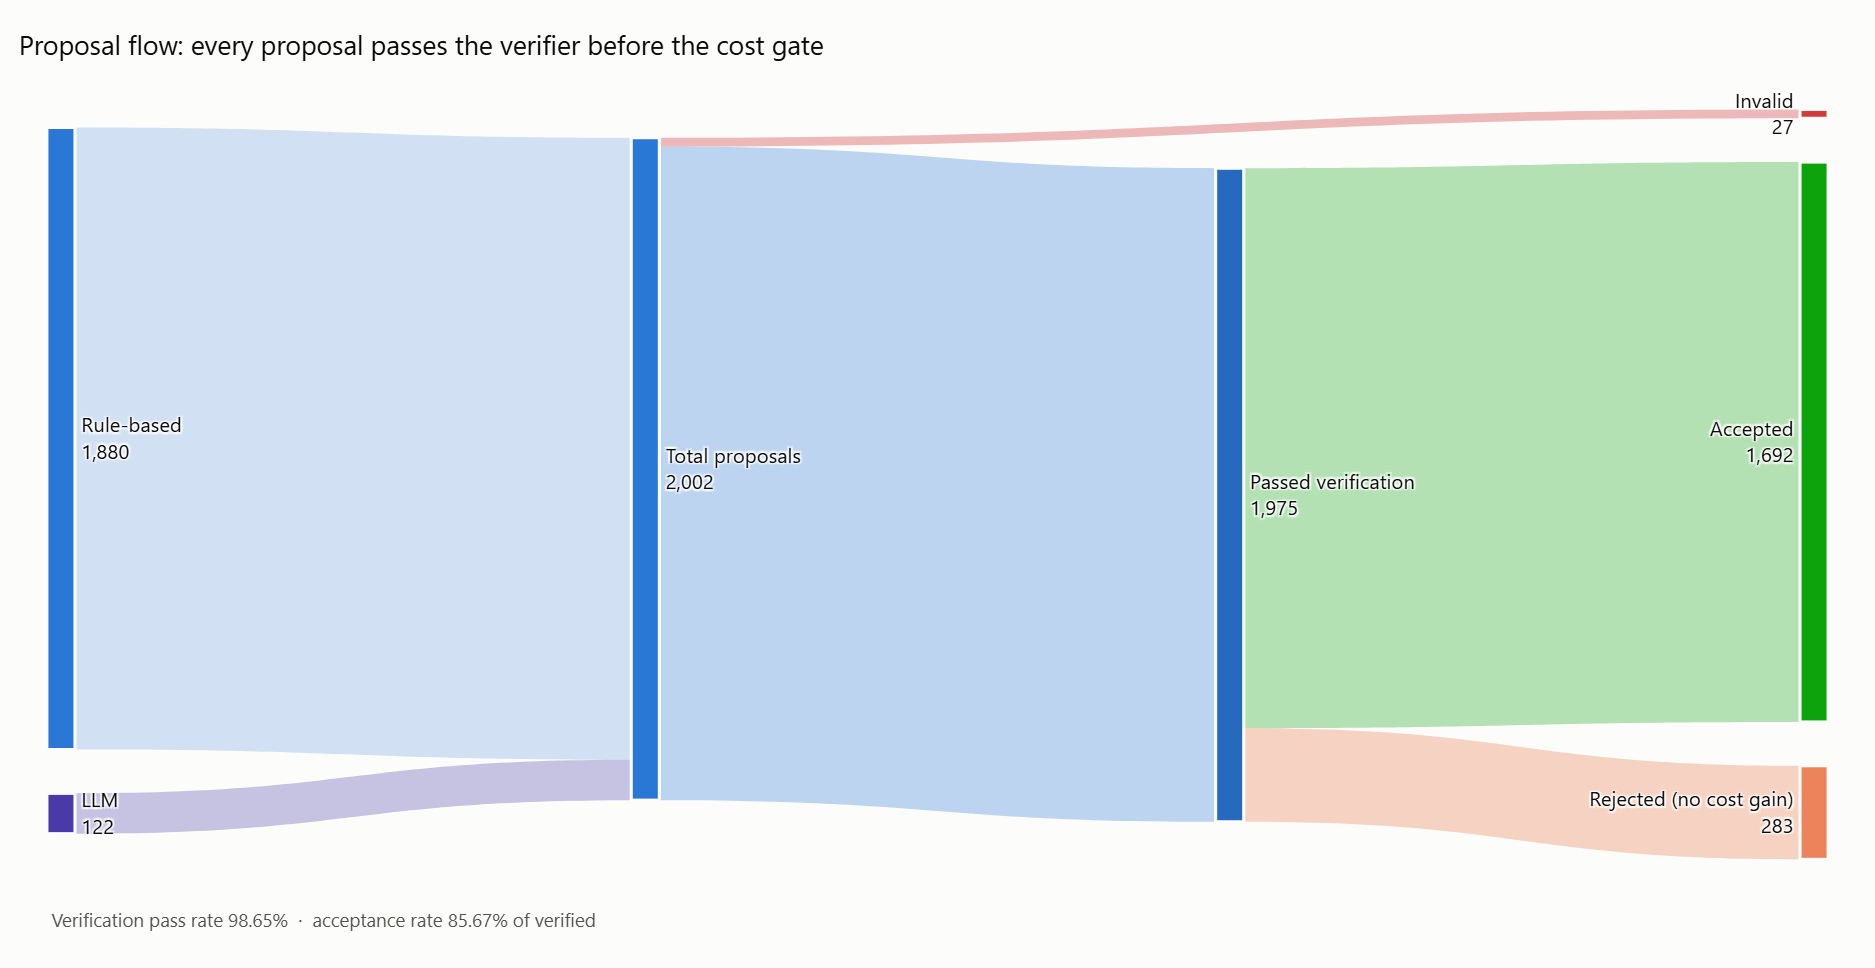
\includegraphics[width=\textwidth]{report_figures/real_sankey_groq.png}
\caption{Real-program sample, rules + Groq: where the proposals went}
\end{figure}

\section{Performance Analysis}

\textbf{The verifier is mandatory:} Of the proposals that could be parsed, 7.6\% of Gemini's, 1.9\% of Groq's and 57\% of the local model's were wrong. Without the verification gate these would have become silent bugs. Because the verifier caught every one, the output of all four runs is sound.

\textbf{LLMs and rules are complementary:} The rule engine is fast and deterministic for standard tasks. Copy propagation alone accounts for about 60\% of all accepted changes, acting as a cleanup step after other passes. The LLMs, conversely, shine on collapsing control flow, which no rule in our set can do.

\textbf{A weak model is still safe:} The local model's low validity rate did not make the results worse, only slower. This is the main practical consequence of verifying every proposal: the choice of model affects how much is gained, never whether the result is correct.

\textbf{Cost gating prevents regression:} Several proposals preserved semantics but did not lower the weighted cost (for example, replacing a multiplication by an equally expensive addition). The Cost Evaluator rejected these zero-gain proposals.

\textbf{Free-tier limits are manageable:} Both cloud providers limit requests and tokens per day. The system spaces its calls, waits out per-minute limits, and for Groq moves to another model when one quota is spent, so a full run completes without supervision.

\textbf{Real programs leave less to remove:} A generated program is mostly constants and collapses to a few prints. A real program computes with its input, so the instructions that do the work have to stay, and the gain comes from cleaning up the translation and the occasional redundancy the programmer left.

\textbf{A proof is stronger than a test:} For programs without loops, zero false positives is no longer a statement about the inputs that were tried. For the programs the solver decided, no input exists on which the optimized program behaves differently.

\textbf{Tests can be passed by a wrong change:} The one wrong change that the re-check found had passed 388 tests. Testing is only as good as its inputs; the lasting answers are inputs chosen to reach behaviour the program shows rarely, an independent re-check of every run, and a proof wherever one is possible.

\textbf{Self-repair helps with form more than with logic:} A capable model that is rejected has usually written a whole expression in one instruction; told so, it answers again in valid TAC. A small local model that got the logic wrong tends to get it wrong again, or to play safe and return the program unchanged.

\section{Limitations}

\begin{itemize}[leftmargin=2cm]
  \item The front end accepts only a subset of C: no arrays, pointers, functions other than \texttt{main}, floating point, or input read inside a loop. That is why only 2\% of the submissions examined could be used.
  \item The SMT stage does not handle loops. Programs with loops are verified by differential testing, which is thorough but is not a proof.
  \item Integers are unbounded in TAC, so the 32-bit wrap-around of C is not modelled, and inputs are tested over the verifier's ranges, which include values a problem statement rules out.
  \item Execution time is an abstract count of cycles from a fixed latency table, measured on 25 inputs. It orders programs sensibly but is not a measurement on real hardware.
  \item The LLM runs on the real programs cover a sample of 100 programs, not all 500; the runs are resumable and can be extended.
\end{itemize}

% ============================================================
\newpage
\begin{thebibliography}{9}

\bibitem[Aho et al., 2006]{aho2006compilers}
Aho, A.\,V., Lam, M.\,S., Sethi, R., \& Ullman, J.\,D. (2006). \textit{Compilers: Principles, Techniques, and Tools} (2nd ed.). Pearson.

\bibitem[Cummins et al., 2022]{cummins2022compilergym}
Cummins, C., Wasti, B., Guo, J., Cui, B., Ansel, J., Gomez, S., \ldots \& Leather, H. (2022). CompilerGym: Robust, performant compiler optimization environments for AI research. \textit{CGO 2022}, 92--105.

\bibitem[Cummins et al., 2024]{cummins2024llmcompiler}
Cummins, C., Seber, V., Commesçon, D., Palermo, J., Leather, H., \& Steiner, B. (2024). Meta Large Language Model Compiler: Foundation models of compiler optimization. \textit{arXiv preprint arXiv:2407.02524}.

\bibitem[Necula, 2000]{necula2000tv}
Necula, G.\,C. (2000). Translation validation for an optimizing compiler. \textit{PLDI 2000}, 83--94.

\bibitem[Phothilimthana et al., 2016]{phothilimthana2016stoke}
Phothilimthana, P.\,M., Thakur, A., Bodik, R., \& Dhurjati, D. (2016). Scaling up superoptimization. \textit{ASPLOS 2016}, 297--310.

\bibitem[de Moura and Bj{\o}rner, 2008]{demoura2008z3}
de Moura, L., Bj{\o}rner, N. (2008). Z3: An efficient SMT solver. \textit{Tools and Algorithms for the Construction and Analysis of Systems (TACAS)}, 337--340.

\bibitem[open-r1, 2025]{openr1codeforces}
open-r1 (2025). \textit{codeforces-submissions} (dataset, CC-BY-4.0). Hugging Face.

\end{thebibliography}

\end{document}
